\documentclass[a4paper,14pt]{extarticle}
% Thay doi chieu cao cua header va top margin
% de fix warning `\headheight is too small`
\setlength{\headheight}{17pt}
\addtolength{\topmargin}{-3pt}

% Package render ngon ngu tieng Viet
\usepackage[utf8]{vietnam}

% Package can le tren, duoi, trai, phai
\usepackage[left=3.5cm,right=2.5cm,top=3cm,bottom=3cm]{geometry}

% Packages de viet cong thuc Toan hoc
\usepackage{amsmath,amssymb, amsthm}
% Package de viet in dam cong thuc Toan hoc (bm = bold math)
\usepackage{bm}

% Package su dung de giu figure/table o dung vi tri
% \begin{figure}[H]
%     ... figure contents...
% \end{figure}
% Note: can check lai (comment ko thay khac biet)
\usepackage{float}

% Package de su dung duoc `subfigure`
\usepackage{subfigure}

% Package custom style cua caption
% (kich thuoc font chu, khoang cach so voi anh, ...)
\usepackage[font=small,skip=0pt]{caption}

% Package custom khoang cach
% giua cac gach dau dong trong danh sach
\usepackage{enumitem}
\setlist{nosep}

% Custom khoang cach giua cac dong (gian dong)
% Note: can check lai dong `usepackage` (comment ko thay khac biet)
\usepackage{setspace}
\renewcommand{\baselinestretch}{1.25}

% Package su dung font Times la font cho text va
% cung cap mot so syntax Toan hoc
\usepackage{mathptmx}

% Package su dung de reference/citation co the click
\usepackage{hyperref}

% Package su dung cho viec danh `chi muc tu khoa`
\usepackage{imakeidx}
\makeindex[columns=2, columnsep=0.5em, title=Chỉ mục từ khoá, intoc]

% Package su dung cho `khungtrangbia`
\usepackage{tikz}

% Package su dung cho `pythoncodestyle`
\usepackage{listings}

% Package su dung cho `headerfooterstyle`
\usepackage{fancyhdr}

% Custom style cho header and footer
% De su dung duoc custom style nay, can `\usepackage{fancyhdr}`
\def\headerfooterstyle{
    \pagestyle{fancy}
    \fancyhf{}
    \lhead{\thesection}
    \rhead{\thepage}
    \lfoot{}
    \rfoot{Nguyễn Hữu Minh}
    \renewcommand{\headrulewidth}{2pt}
    \renewcommand{\footrulewidth}{1pt}
}

\headerfooterstyle

% Package su dung de ve bang `tab_result` trong file `4_munit_results.tex`
\usepackage[flushleft]{threeparttable}

% Package su dung de dung `tab` \tab
\usepackage{tabto}

% Khai bao ky tu unicode de sua error
% Package inputenc: Unicode character − (U+2212) (inputenc) not set up for use with LaTeX.
\DeclareUnicodeCharacter{2212}{-}

\begin{document}

    % BAT DAU CAC TRANG CHUC NANG
    % Xoa page number
    \pagenumbering{gobble}
    % Xoa header - footer
    \pagestyle{plain}

    
\def\trangbia{
    % % De dung "khung_trang_bia", ta can `\usepackage{tikz}`
    % 
% De su dung "khungtrangbia", ta can `\usepackage{tikz}`
\def\khungtrangbia{
  \begin{tikzpicture}[remember picture,overlay,inner sep=0,outer sep=0]
    \draw[black!70!black,line width=3pt]([xshift=-2cm,yshift=-2.5cm]current page.north east)
    coordinate (A) -- ([xshift=2.5cm,yshift=-2.5cm]current page.north west)
    coordinate (B) -- ([xshift=2.5cm,yshift=2.5cm]current page.south west)
    coordinate (C) -- ([xshift=-2cm,yshift=2.5cm]current page.south east)
    coordinate (D) -- cycle;
    \draw ([yshift=0.5cm,xshift=-0.5cm]A) --
    ([yshift=0.5cm,xshift=0.5cm]B) --
    ([yshift=-0.5cm,xshift=0.5cm]B) --
    ([yshift=-0.5cm,xshift=-0.5cm]B) --
    ([yshift=0.5cm,xshift=-0.5cm]C) --
    ([yshift=0.5cm,xshift=0.5cm]C) --
    ([yshift=-0.5cm,xshift=0.5cm]C) --
    ([yshift=-0.5cm,xshift=-0.5cm]D) --
    ([yshift=0.5cm,xshift=-0.5cm]D) --
    ([yshift=0.5cm,xshift=0.5cm]D) --
    ([yshift=-0.5cm,xshift=0.5cm]A) --
    ([yshift=-0.5cm,xshift=-0.5cm]A) --
    ([yshift=0.5cm,xshift=-0.5cm]A);
    \draw ([yshift=-0.3cm,xshift=0.3cm]A) --
    ([yshift=-0.3cm,xshift=-0.3cm]B) --
    ([yshift=0.3cm,xshift=-0.3cm]B) --
    ([yshift=0.3cm,xshift=0.3cm]B) --
    ([yshift=-0.3cm,xshift=0.3cm]C) --
    ([yshift=-0.3cm,xshift=-0.3cm]C) --
    ([yshift=0.3cm,xshift=-0.3cm]C) --
    ([yshift=0.3cm,xshift=0.3cm]D) --
    ([yshift=-0.3cm,xshift=0.3cm]D) --
    ([yshift=-0.3cm,xshift=-0.3cm]D) --
    ([yshift=0.3cm,xshift=-0.3cm]A) --
    ([yshift=0.3cm,xshift=0.3cm]A) --
    ([yshift=-0.3cm,xshift=0.3cm]A);
  \end{tikzpicture}
}

    % \vekhungtrangbia
    
    \large {\bf \centerline {TRƯỜNG ĐẠI HỌC BÁCH KHOA HÀ NỘI}}
    \vskip 0.6in

    % \begin{center}
    %     
\includegraphics[width=0.25\columnwidth]{images/logo_bk.png}
    % \end{center}
    \vskip 0.5in

    \LARGE {\bf \centerline {LUẬN VĂN THẠC SĨ}}
    \vskip 0.6in

    \LARGE {\bf \centerline {Ứng dụng mô hình học sâu}}
    \LARGE {\bf \centerline {giải quyết một số bài toán}}
    \LARGE {\bf \centerline {phân tích và xử lý hình ảnh}}
    \vskip 0.6in

    \hspace{3cm}
    \normalsize {\bf NGUYỄN HỮU MINH}
    \vskip 0in
    \hspace{3cm}
    \normalsize {}
    \vskip 0in
    \hspace{3cm}
    \normalsize {\textbf{Ngành}: Toán Tin}
    \vskip 0in
    \hspace{3cm}
    \normalsize {\textbf{Chuyên ngành}: Toán Tin}
    \vskip 1.3in

    \hspace{0.5cm}
    \small {\textbf{Giảng viên hướng dẫn}: ......................................}
    \hspace{0.5cm}
    \begin{tikzpicture}
        \draw (15.5,0)--(18.5,0);
    \end{tikzpicture}
    \vskip 0in

    \hspace{0.5cm}
    \small {\textbf{Bộ môn}: Toán Tin \hspace{5.7cm} Chữ ký của GVHD}
    \vskip 0in

    \hspace{0.5cm}
    \small {\textbf{Viện}: Toán ứng dụng và Tin học}
    \vskip 1.2in
  
    \small {\centerline {Hà Nội, 06/2020}}
}

    \trangbia

    \newpage
    
\def\nhanxet{
    \large {\bf {\centerline {NHẬN XÉT CỦA GIẢNG VIÊN HƯỚNG DẪN}}}
    \vskip 0.5in

    \normalsize {\bf \flushleft{1. Mục đích và nội dung của đồ án:}}
    \vskip 2in

    \normalsize {\bf \flushleft{2. Kết quả đạt được:}}
    \vskip 2in

    \normalsize {\bf \flushleft{3. Ý thức làm việc của sinh viên:}}
    \vskip 2in

    \hspace{8cm}
    \normalsize {Hà Nội, ngày \hspace{0.5cm} tháng \hspace{0.5cm} năm}
    \vskip 0in

    \hspace{8.5cm}
    \normalsize {\textit{Giảng viên hướng dẫn}}
}

    \nhanxet

    \newpage
    
\def\loicamon{
    \section*{Lời cảm ơn}
    \addcontentsline{toc}{section}{Lời cảm ơn}
    Với tấm lòng biết ơn vô cùng sâu sắc, tôi xin gửi lời cảm ơn chân thành nhất đến quý Thầy Cô của Viện Toán ứng dụng và Tin học, Đại học Bách Khoa Hà Nội đã tạo điều kiện và dành cho tôi vốn kiến thức quý báu. \\
    Đặc biệt, tôi xin chân thành cảm ơn ThS. --------- đã tận tâm hướng dẫn tôi trong suốt thời gian vừa qua.
    Nhờ có những lời hướng dẫn của thầy mà luận văn của tôi đã hoàn thành một cách tốt nhất. \\
    Tôi rất mong nhận được ý kiến đóng góp của quý Thầy Cô và các bạn học để luận văn của ôi được hoàn thiện hơn.
    Tôi xin chân thành cảm ơn!
}

    \loicamon

    % Bat dau danh so trang page number
    \pagenumbering{arabic}

    \newpage
    
\def \tomtatnoidung{
    \section*{Tóm tắt nội dung đồ án}
    \addcontentsline{toc}{section}{Tóm tắt nội dung đồ án}
    Cách mạng công nghiệp 4.0 đã mang đến cho con người một kỷ nguyên khai phá dữ liệu. Điều này đặt ra bài toán không chỉ làm sao để khai phá được dữ liệu một cách hiệu quả mà còn làm sao để sinh ra được thêm nhiều dữ liệu một cách tự động và với số lượng lớn. Do đó, trong khuôn khổ của đồ án tốt nghiệp, em sẽ nghiên cứu về ý tưởng chung, kiến trúc, hàm loss, phương pháp đánh giá, những vấn đề tồn đọng và cách giải quyết các vấn đề đó của mô hình Generative Adversarial Networks (GANs) tổng quát nhằm giải quyết bài toán sinh dữ liệu ảnh nói và mô hình Multimodal Unsupervised Image-to-Image Translation (MUNIT) giúp giải quyết bài toán sinh dữ liệu ảnh mới từ ảnh đã có sẵn (Image-to-Image Translation). Bên cạnh những kết quả đã được công bố trong bài báo, em đã thử nghiệm mô hình với bộ dữ liệu khác để chứng minh tính đúng đắn của mô hình và lấy đó làm tiền đề cho việc phát triển những mô hình phức tạp hơn trong tương lai.
    \vskip 2.5in

    \hspace{7.7cm}
    \normalsize {Hà Nội, ngày \hspace{0.5cm} tháng \hspace{0.5cm} năm}
    \vskip 0in

    \hspace{8.5cm}
    \normalsize {\textit{Sinh viên thực hiện}}
}
    \tomtatnoidung

    \newpage
    \tableofcontents

    \newpage
    \listoffigures
    \addcontentsline{toc}{section}{Danh sách hình vẽ}

    \newpage
    \listoftables
    \addcontentsline{toc}{section}{Danh sách bảng biểu}
    % KET THUC CAC TRANG CHUC NANG

    % BAT DAU PHAN NOI DUNG CHINH
    % Bat dau hien header - footer tu trang nay ve sau
    \pagestyle{fancy}

    \newpage
    \def\cacbaitoan{
    \section{Nhóm bài toán về khuôn mặt}
    \subsection{Bài toán Object Detection và Object Detection trong ảnh chất lượng cao}
    Mặc dù bài toán Object Detection rất phổ biến và được coi là một trong số các bài toán deep learning kinh điển, nhưng vẫn tồn tại những vấn đề nan giải và đến nay vẫn là chủ đề hot trong giới nghiên cứu, đó chính là bài toán Object Detection với ảnh chất lượng cao.
    \subsection{Bài toán Face Detection}
    - Dựa trên các nghiên cứu trong TinaFace => dẫn dắt sang bài toán Face Detection
    
    \subsection{Bài toán Face Recognition}
    % \subsection{Phát biểu bài toán phân loại Face Attributes}
}
    \cacbaitoan

    \newpage
    \def\objectdetection{
    \section{Các mô hình giải quyết bài toán Object Detection}
    \subsection{Các mô hình two-stage giải quyết bài toán Object Detection}
    Các mô hình two-stage giải quyết bài toán Object Detection có đặc điểm chung về kiến trúc mô hình gồm hai phần: \\
    - Phần thứ nhất được gọi là \textit{Region proposals module}, mô đun nhận đầu vào là ảnh ban đầu và trả đầu ra giúp đề xuất ra các khu vực trên ảnh mà có khả năng chứa object. \\
    - Phần thứ hai được gọi là \textit{Feature extraction module}, mô đun nhận đầu vào là kết quả của Region proposals module giúp xác định chính xác object trong khu vực đó là object nào và tinh chỉnh toạ độ của khu vực chính xác hơn. \\
    Nổi bật trong nhóm các mô hình two-stage là chuỗi các mô hình R-CNN, Fast R-CNN và Faster R-CNN.

    \subsubsection{Mô hình R-CNN}
        Một trong các mô hình đầu tiên ứng dụng deep learning giải quyết bài toán Object Detection là Regions with CNN features \cite{girshick2014rich} (gọi tắt là R-CNN).
        Tuy nhiên, ở thời điểm mà mô hình R-CNN ra đời, do các mô hình deep learning chưa thật sự phát triển nên mô hình R-CNN không hoàn toàn sử dụng deep learning mà vẫn dựa trên kết quả của thuật toán xử lý ảnh như Graph-Based Image Segmentation \cite{felzenszwalb2004efficient} và Selective Search \cite{uijlings2013selective}.
        \noindent
        \textbf{\textit{Thuật toán Graph-Based Image Segmentation}} \\
        \noindent
        \textbf{\textit{Thuật toán Selective Search}} \\
        
        \noindent
        \textbf{\textit{Kiến trúc mô hình R-CNN}} \\
        Là một trong số các mô hình two-stage, mô hình R-CNN bao gồm hai thành phần: \\
        - Phần Region proposals module mà mô hình R-CNN sử dụng là thuật toán Selective Search ở trên.
        Nhận đầu vào là ảnh, thuật toán Selective Search trả đầu ra là khoảng 2000 khu vực và mô hình R-CNN sử dụng các khu vực này làm đầu vào cho thành phần thứ hai. \\
        - Phần Feature extraction module của mô hình R-CNN là một mô hình phân lớp ảnh, cụ thể theo \cite{girshick2014rich} là AlexNet.
        Mô hình R-CNN sử dụng AlexNet nhằm đánh giá xem khu vực đã được đề xuất bởi Selective Search có chứa object hay không và nếu có thì khu vực đó chứa object nào. \\

        \begin{figure}[H]
            \centering
            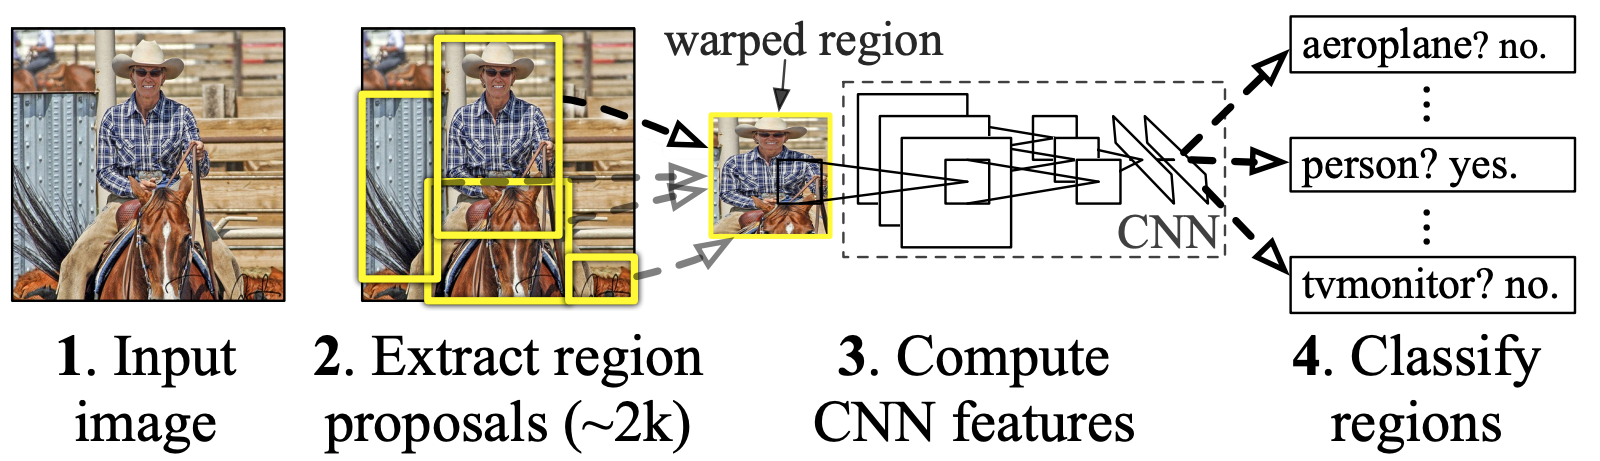
\includegraphics[width=13cm] {images/rcnn_model}
            \caption{Kiến trúc mô hình R-CNN (Nguồn: \cite{girshick2014rich})}
            \label{fig:rcnn_model}
        \end{figure}

        \noindent
        Đến đây, nhóm tác giả thực hiện hai bước: \\
        \textit{Bước 1}: Finetune mô hình phân lớp CNN \\
        Nhóm tác giả thay thế lớp fully-connected cuối cùng của mô hình AlexNet (gồm 1000 lớp theo bộ dữ liệu ImageNet) bằng một lớp fully-connected mới (gồm 21 lớp: 20 lớp của bộ dữ liệu VOC và 1 lớp ứng với background).
        Và họ finetune lại mô hình này với thuật toán tối ưu là SGC và learning rate rất nhỏ.
        Các khu vực đã được đề xuất bởi thuật toán Selective Search được sử dụng làm dữ liệu cho bước này, trong đó: \\
        - Những khu vực có chỉ số IoU với groundtruth bounding box >= 0.5 sẽ được gán nhãn là lớp của bounding box đó. \\
        - Những khu vực không có chỉ số IoU với bất kỳ groundtruth bounding box nào >= 0.5 sẽ được gán nhãn là lớp background. \\
        TODO Appendix B \\
        Lý do ta cần có bước finetune này được nhóm tác giả giải thích rằng có những điểm khác nhau giữa bộ dữ liệu gốc ImageNet đã được train cho mô hình AlexNet và bộ dữ liệu gồm các khu vực được đề xuất bởi Selective Search.
        Hiệu quả của việc finetune này sẽ được nói đến ở dưới đây. \\
        \textit{Bước 2}: Xây dựng bộ phân lớp object bằng SVM \\
        Với mô hình AlexNet đã được finetune lại như trên, nhóm tác giả sử dụng nó để lấy ra các đặc trưng của ảnh đầu vào và từ đó train các mô hình SVM.
        Mỗi mô hình SVM tương ứng với một lớp đối tượng và mỗi mô hình SVM trả lời cho câu hỏi, đặc trưng của khu vực đó có phải là object đó hay không.
        Những đặc trưng của khu vực có chỉ số IoU với groundtruth bounding box >= 0.3 sẽ được gán nhãn là lớp của bounding box đó.
        Và ngược lại, những đặc trưng của khu vực có chỉ số IoU với groundtruth bounding box < 0.3 sẽ được gán nhãn không phải là lớp của bounding box đó. \\
        TODO Appendix B \\
        \textit{Bước 3 (Tuỳ chọn)}: Bổ sung thêm hàm loss cải thiện khả năng định vị khu vực \\
        TODO Appendix C \\

        \noindent
        \textbf{\textit{Kết quả của mô hình R-CNN}} \\
        Kết quả của mô hình R-CNN trên bộ dữ liệu VOC 2010 test rất đáng chú ý.
        Trong hình \ref{fig:rcnn_results_3}, ta xét đến hai cấu hình của mô hình R-CNN: \\
        - Cấu hình cơ bản không bao gồm bước Bổ sung thêm hàm loss cải thiện khả năng định vị khu vực được gọi là R-CNN. \\
        - Cấu hình nâng cao Bổ sung thêm hàm loss cải thiện khả năng định vị khu vực được gọi là R-CNN BB. \\
        Với cấu hình cơ bản, R-CNN đạt được chỉ số average precision cao hơn trên tất cả các lớp đối tượng và chỉ số mAP cao hơn 10\% so với các mô hình hiện đại nhất tại thời điểm đó.
        Hơn nữa, với cấu hình R-CNN BB, mô hình còn đạt được chỉ số AP trên tất cả các lớp đối tượng và chỉ số mAP cao hơn 3\% so với cấu hình cơ bản R-CNN.
        \begin{figure}[H]
            \centering
            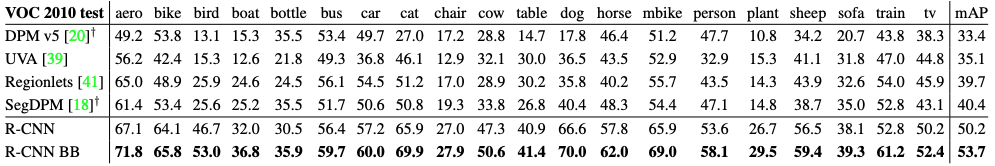
\includegraphics[width=15cm] {images/rcnn_results_3}
            \caption{Kết quả của mô hình R-CNN trên bộ dữ liệu VOC 2010 test. So sánh kết quả của R-CNN và của các mô hình khác nhau (Nguồn: \cite{girshick2014rich})}
            \label{fig:rcnn_results_3}
        \end{figure}
        \noindent
        Ngoài ra, nhóm tác giả cũng nghiên cứu kết quả giữa các cấu hình khác nhau của mô hình R-CNN.
        Trong hình \ref{fig:rcnn_results_1}, nhóm tác giả xét đến hai nhóm cấu hình khác nhau: \\
        - Nhóm cấu hình không finetune và sử dụng đặc trưng ở các vị trí khác nhau cho mô hình phân lớp SVM: \par
        + Cấu hình lấy đặc trưng ở lớp pooling thứ 5: R-CNN ${pool}_{5}$. \par
        + Cấu hình lấy đặc trưng ở lớp fully-connected thứ 6: R-CNN ${fc}_{6}$. \par
        + Cấu hình lấy đặc trưng ở lớp fully-connected thứ 7: R-CNN ${fc}_{7}$. \\
        - Nhóm cấu hình có finetune và sử dụng đặc trưng ở các vị trí khác nhau cho mô hình phân lớp SVM: \par
        + Cấu hình lấy đặc trưng ở lớp pooling thứ 5: R-CNN FT ${pool}_{5}$. \par
        + Cấu hình lấy đặc trưng ở lớp fully-connected thứ 6: R-CNN FT ${fc}_{6}$. \par
        + Cấu hình lấy đặc trưng ở lớp fully-connected thứ 7: R-CNN FT ${fc}_{7}$. \par
        + Cấu hình lấy đặc trưng ở lớp fully-connected thứ 7 kết hợp với hàm loss cải thiện khả năng định vị khu vực: R-CNN FT ${fc}_{7}$ BB. \\
        Với việc finetune lại mô hình với dữ liệu VOC, nhóm cấu hình có finetune mang lại kết quả tốt hơn rất nhiều.
        Trong việc lựa chọn vị trí lấy đặc trưng, vị trí lớp fully-connected thứ 6 là tốt nhất trong nhóm các mô hình không finetune.
        Còn đối với nhóm các mô hình có finetune, vị trí lớp fully-connected thứ 7 là mô hình có kết quả tốt nhất.
        Kết hợp tất cả các kết quả trên, cấu hình R-CNN FT ${fc}_{7}$ BB cho kết quả tốt nhất so sánh với tất cả các cấu hình khác.
        \begin{figure}[H]
            \centering
            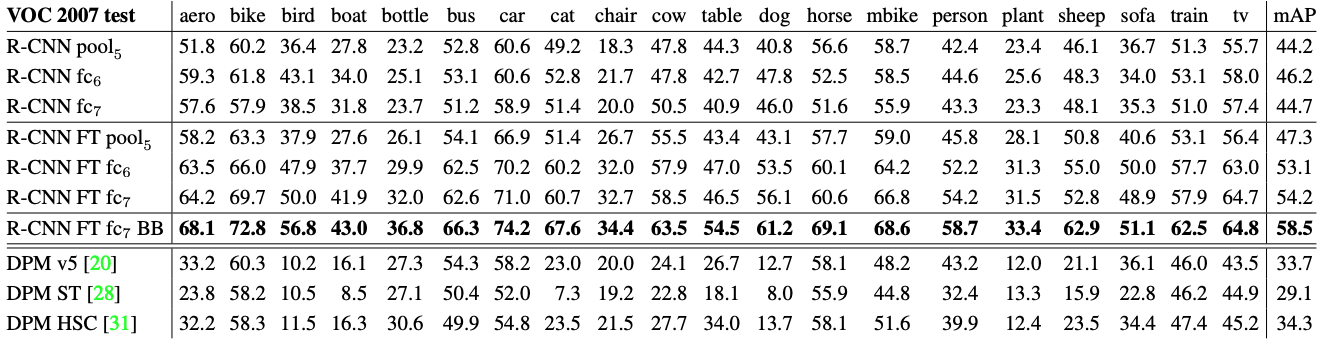
\includegraphics[width=15cm] {images/rcnn_results_1}
            \caption{Kết quả của mô hình R-CNN trên bộ dữ liệu VOC 2007 test. So sánh kết quả của các cấu hình khác nhau của mô hình R-CNN và của mô hình DPM (Nguồn: \cite{girshick2014rich})}
            \label{fig:rcnn_results_1}
        \end{figure}
        \noindent
        Cuối cùng, nhóm tác giả so sánh vai trò của Feature extraction module đối với kết quả chung của mô hình R-CNN.
        Trong hình \ref{fig:rcnn_results_2}, nhóm tác giả xét đến hai mô hình có thể sử dụng trong Feature extraction module: \\
        - Cấu hình sử dụng mô hình AlexNet: R-CNN T-Net và R-CNN T-Net BB. \\
        - Cấu hình sử dụng mô hình VGG16: R-CNN O-Net và R-CNN O-Net BB. \\
        Trong thí nghiệm này, mô hình VGG16 cho kết quả tốt hơn khá nhiều so với mô hình AlexNet.
        \begin{figure}[H]
            \centering
            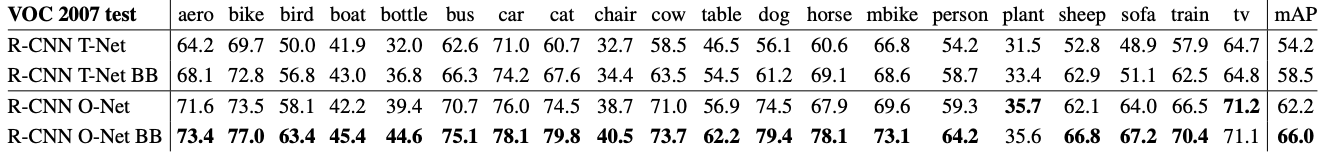
\includegraphics[width=15cm] {images/rcnn_results_2}
            \caption{Kết quả của mô hình R-CNN trên bộ dữ liệu VOC 2007 test (Nguồn: \cite{girshick2014rich})}
            \label{fig:rcnn_results_2}
        \end{figure}

        \noindent
        \textbf{\textit{Vấn đề tồn đọng của mô hình R-CNN}} \\
        Vấn đề lớn nhất của mô hình R-CNN là thời gian mà mô hình cần cho quá trình train và quá trình test là rất lớn.
        Trong quá trình test, mô hình R-CNN sử dụng tới 47 giây để hoàn thành việc xử lý một ảnh.
        Kết quả này khiến cho mô hình R-CNN gần như không có giá trị thực tiễn.

    \subsubsection{Mô hình Fast R-CNN}
        Fast R-CNN \cite{girshick2015fast}, được phát triển bởi một trong nhóm tác giả của mô hình R-CNN, và là một mô hình nâng cấp hơn so với R-CNN giúp phần nào giải quyết được một phần điểm yếu về tốc độ của mô hình R-CNN.
        \noindent
        \textbf{\textit{Kiến trúc mô hình Fast R-CNN}} \\
        Là một phiên bản nâng cấp của mô hình R-CNN, nên Fast R-CNN cũng bao gồm hai thành phần: \\
        - Phần Region proposals module mà mô hình Fast R-CNN sử dụng vẫn là thuật toán Selective Search tương tự như R-CNN. \\
        - Phần Feature extraction module của mô hình R-CNN là một mô hình phân lớp ảnh, cụ thể theo \cite{girshick2015fast} là VGG16. \\
        Các thành phần của mô hình Fast R-CNN không có thay đổi gì quá nổi bật so với R-CNN, tuy nhiên, điểm khác biệt mang lại giá trị của Fast R-CNN nằm ở cách mà mô hình này kết hợp hai thành phần trên.
        \begin{figure}[H]
            \centering
            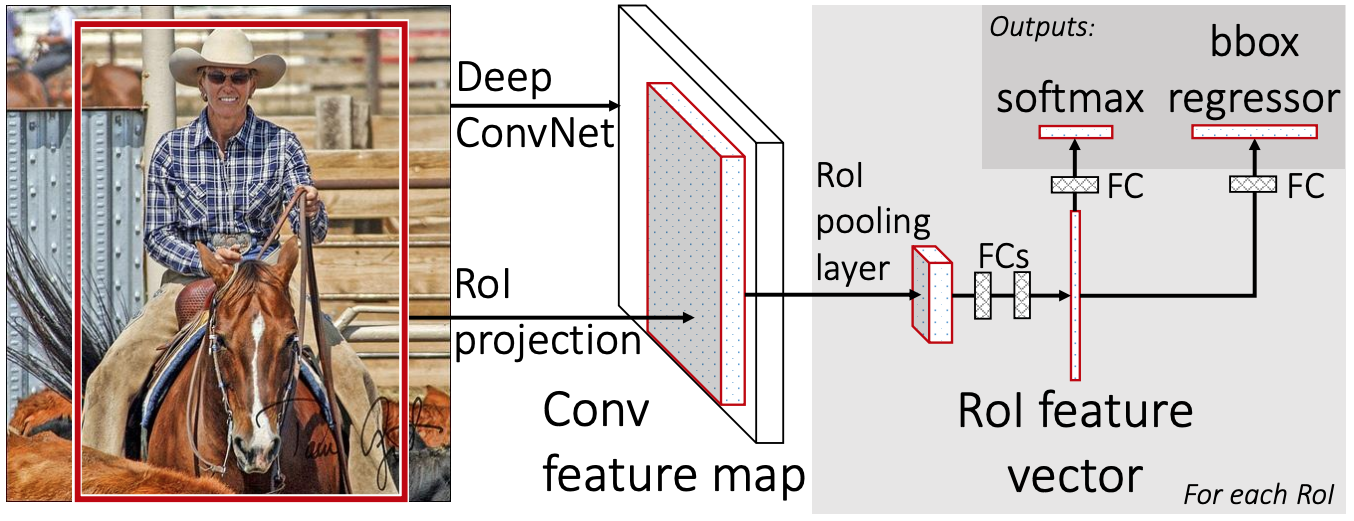
\includegraphics[width=13cm] {images/fast_rcnn_model}
            \caption{Kiến trúc mô hình Fast R-CNN (Nguồn: \cite{girshick2015fast})}
            \label{fig:fast_rcnn_model}
        \end{figure}
        \noindent
        Khác với R-CNN, mô hình Fast R-CNN đưa toàn bộ ảnh ban đầu qua các lớp conv và pooling của Feature extraction module để tạo ra được đặc trưng của toàn bộ ảnh.
        Tiếp theo, với mỗi khu vực mà thuật toán Selective Search đề xuất (các khu vực này, theo \cite{girshick2015fast}, gọi là các \textit{regions of interest} hay \textit{RoIs}), mô hình Fast R-CNN trích xuất từ đặc trưng của toàn bộ ảnh ra đặc trưng đại diện cho khu vực đề xuất đó.
        Cuối cùng, mỗi đặc trưng đại diện cho mỗi khu vực đề xuất được đưa qua các lớp fully-connected và trả hai đầu ra gồm giá trị xác suất khu vực đó là đối tượng nào và giá trị độ lệch của bounding box. \\
        Tuy nhiên, có một vấn xảy ra với cách thiết kế mô hình trên, đó là mỗi khu vực đề xuất từ thuật toán Selective Search có kích thước khác nhau, do đó, kích thước của đặc trưng đại diện cho mỗi khu vực đề xuất cũng khác nhau và ta cần các đặc trưng này có cùng kích thước để có thể đưa vào cùng chung các lớp fully-connected.
        Tác giả giải quyết vấn đề này bằng cách xây dựng một lớp mới trong kiến trúc mô hình Fast R-CNN, tên là \textit{RoI pooling}. \\

        \textbf{\textit{Lớp RoI pooling}} \\
        Trước khi đi sâu vào chi tiết của lớp RoI pooling, ta sẽ cùng bàn luận về lớp pooling thông thường.
        Có hai phương pháp pooling phổ biến là max pooling và average pooling.
        \begin{figure}[H]
            \centering
            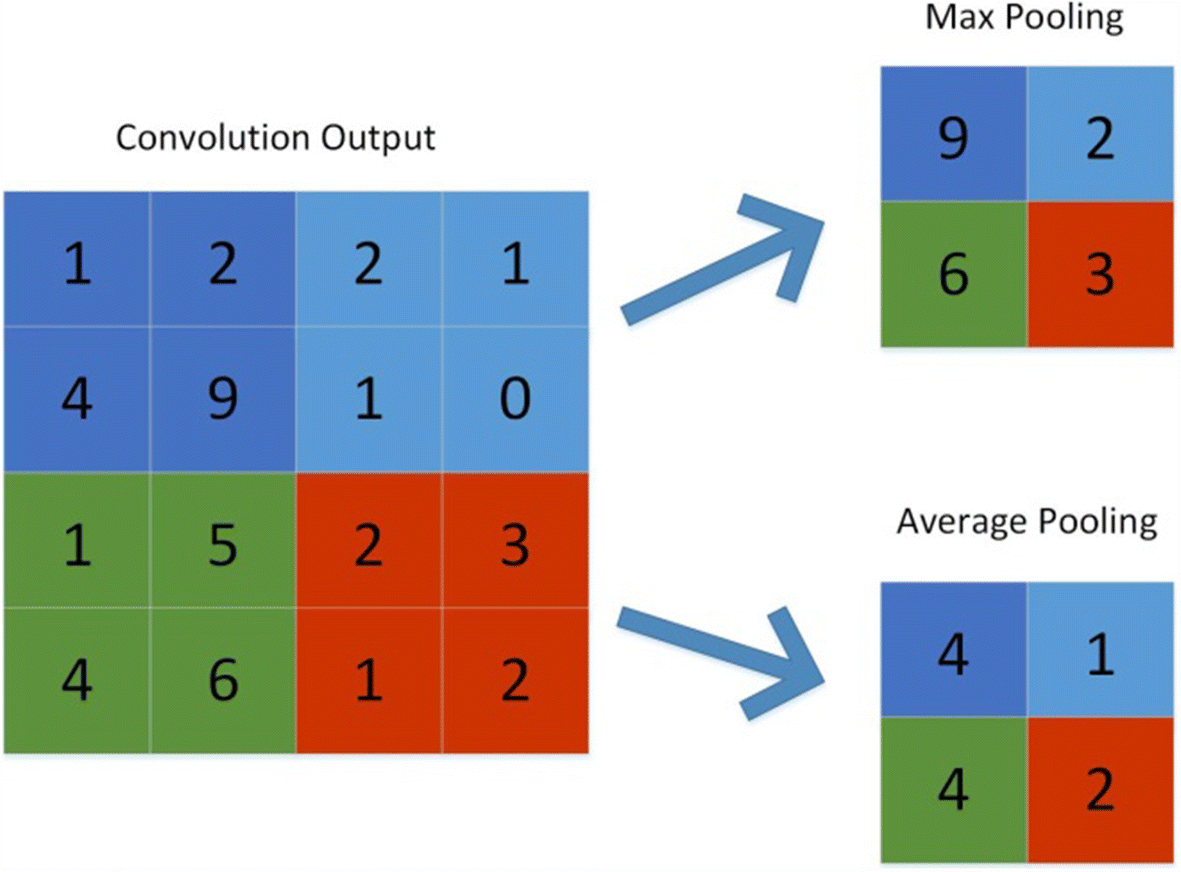
\includegraphics[width=8cm] {images/pooling}
            \caption{Kết quả sau khi thực hiện max pooling và average pooling (Nguồn: media.springernature.com)}
            \label{fig:pooling}
        \end{figure}

        \noindent
        Tuy nhiên, hai phương pháp trên đều có cách thực hiện dựa trên kernel và stride, nghĩa là kích thước của đặc trưng sau khi đi qua lớp pooling phụ thuộc vào kích thước đặc trưng trước khi đi qua lớp pooling, kích thước của kernel pooling và kích thước của stride pooling. \\
        Cụ thể hơn, với một đặc trưng từ lớp conv có kích thước chiều rộng và chiều cao lần lượt là ${W}_{1}$ và ${H}_{1}$ và lớp pooling có kích thước kernel là K, kích thước stride là S, ta sẽ thu được đặc trưng sau khi đi qua lớp pooling này có kích thước chiều rộng và chiều cao lần lượt là ${W}_{2} = \frac{{W}_{1} - (K - 1) - 1}{S} + 1$ và ${H}_{2} = \frac{{H}_{1} - (K - 1) - 1}{S} + 1$.

        \begin{figure}[H]
            \centering
            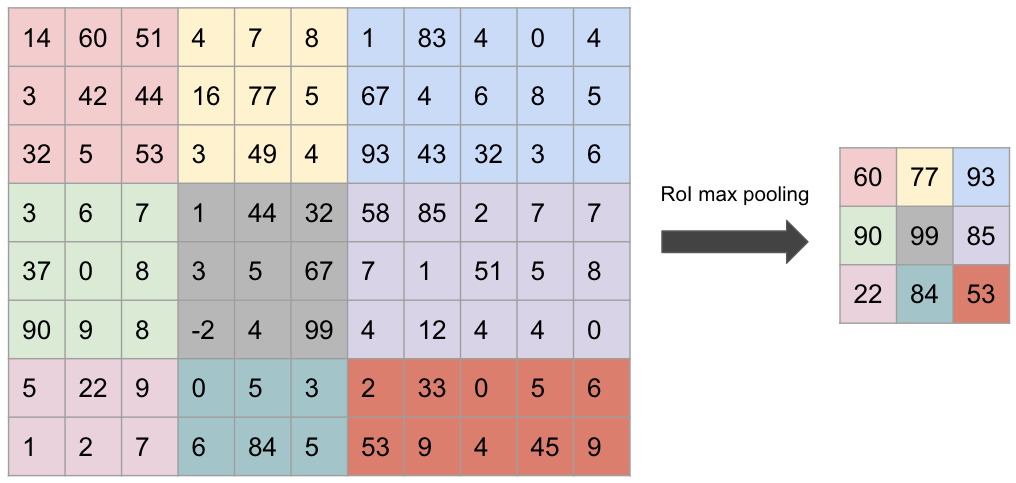
\includegraphics[width=10cm] {images/roi_pooling}
            \caption{Kết quả sau khi thực hiện RoI max pooling}
            \label{fig:roi_pooling}
        \end{figure}

        \noindent
        Trong khi đó, RoIs pooling được giới thiệu bởi tác giả không hoạt động như vậy.
        Thay vì yêu cầu ta phải định nghĩa kích thước kernel và kích thước stride, RoI pooling yêu cầu ta phải định nghĩa kích thước của đặc trưng đầu ra, từ đó, RoI pooling sẽ tính toán và chia đặc trưng đầu vào thành các vùng trước khi thực hiện phép max pooling. \\
        Cụ thể hơn, với một đặc trưng từ lớp conv có kích thước chiều rộng và chiều cao lần lượt là ${W}_{1}$ và ${H}_{1}$ và ta định nghĩa kích thước của đặc trưng đầu ra có kích thước chiều rộng và chiều cao lần lượt là ${W}_{2}$ và ${H}_{2}$, RoI pooling sẽ tính toán được kích thước và vị trí của từng khu vực pooling: \\
        - Theo chiều W, ta có ${W}_{2}$ phần pooling và mỗi phần có kích thước là ${K}_{w} = \lfloor\frac{{W}_{1}}{{W}_{2}}\rfloor$, ngoại trừ phần cuối có kích thước ${K}_{w} + ({W}_{1} - {W}_{2} * {K}_{w})$. \\
        - Theo chiều H, ta có ${H}_{2}$ phần pooling và mỗi phần có kích thước là ${K}_{h} = \lfloor\frac{{H}_{1}}{{H}_{2}}\rfloor$, ngoại trừ phần cuối có kích thước ${K}_{h} + ({H}_{1} - {H}_{2} * {K}_{h})$. \\

        \noindent
        \textbf{\textit{Hàm loss multi-task và cách finetune mô hình Fast R-CNN}} \\
        Một điểm cải tiến khác của mô hình Fast R-CNN so với mô hình R-CNN đó là việc sử dụng hàm loss multi-task và finetune toàn bộ mô hình. \\
        Trong quá trình train mô hình, tác giả lấy ngẫu nhiên N ảnh và lấy ngẫu nhiên $\frac{R}{N}$ RoIs trên mỗi ảnh.
        Nhằm đảm bảo vấn đề về bộ nhớ không xảy ra trong suốt quá trình train, tác giả lựa chọn N = 2 và R = 128.
        Ngoài ra, tác giả cũng đề cập đến một lo ngại khác, đó là việc sử dụng nhiều RoIs trên một số ít ảnh có thể dẫn đến quá trình tối ưu chậm và mất nhiều thời gian để mô hình đạt được điểm hội tụ.
        Tuy nhiên, trong thực tế, điều này đã không xảy ra. \\
        Mô hình Fast R-CNN có hai lớp đầu ra: \\
        - Một là giá trị xác suất một khu vực nào đó là đối tượng nào $p = (p_0, \dots, p_K)$, tương ứng với $K + 1$ lớp đối tượng ($K$ lớp đối tượng từ bộ dữ liệu và 1 lớp background). \\
        - Còn lại là giá trị độ lệch bounding box của khu vực đó $t^{k} = (t^{k}_{x}, t^{k}_{y}, t^{k}_{w}, t^{k}_{h})$, tương ứng với $K$ lớp đối tượng từ bộ dữ liệu. \\
        Với groundtruth lớp đối tượng $u$ và groundtruth toạ độ bounding box $v$, ta có hàm loss multi-task với mỗi RoI như sau:
        \begin{equation}
            \label{eq:fast_rcnn_loss}
            L(p, u, t^u, v) = L_{cls}(p, u) + \lambda [u \ge 1] L_{loc}(t^u, v)
        \end{equation}
        Hàm loss trên gồm các thành phần: \\
        Đầu tiên, thành phần $L_{cls}(p, u) = -\log p_u$ là hàm log loss với groundtruth lớp đối tượng $u$ \\
        Tiếp theo, thành phần $[u \ge 1]$ là hàm chỉ định. Thành phần này bằng 1 nếu $u \ge 1$ và bằng 0 trong các trường hợp còn lại. Thành phần này tồn tại nhằm loại bỏ phần hàm loss tính toán độ lệch bounding box nếu lớp đối tượng $u = 0$ bởi vì khi đó, $u$ đại diện cho lớp background. \\
        Cuối cùng, thành phần $L_{loc}(t^u, v)$ là hàm loss tính toán độ lệch giữa groundtruth toạ độ bounding box $v = (v_{x}, v_{y}, v_{w}, v_{h})$ và bounding box dự đoán $t^u = (t^u_{x}, t^u_{y}, t^u_{w}, t^u_{h})$ tương ứng với groundtruth lớp đối tượng $u$. Mỗi bounding box được biểu diễn bởi bốn giá trị, x - toạ độ x của góc trái trên, y - toạ độ y của góc trái trên, w - chiều rộng của bounding box và h - chiều cao của bounding box.
        Công thức cụ thể của thành phần $L_{loc}(t^u, v)$ như sau:
        \begin{equation}
            \label{eq:fast_rcnn_bb_loss}
            L_{loc}(t^u, v) = \sum_{i \in \{{x},{y},{w},{h}\}} {smooth}_{L_1}(t^u_i - v_i),
        \end{equation}
        trong đó:
        \begin{equation}
            \label{eq:fast_rcnn_bb_loss_l1}
            {smooth}_{L_1}(x) =
            \begin{cases}
                0.5x^2& {if} |x| < 1 \\
                |x| - 0.5& {otherwise},
            \end{cases}
        \end{equation}
        Tác giả giải thích việc sử dụng hàm ${smooth}_{L_1}(x)$ bởi vì nó ít nhạy cảm hơn với outliers so với hàm ${L_2}$ được sử dụng trong mô hình R-CNN.
        Ngoài ra, tác giả cũng chuẩn hoá các toạ độ $v$ với trung bình bằng 0 và phương sai đơn vị.
        Giá trị $\lambda$ được tác giả sử dụng nhằm cân bằng giữa hai thành phần loss, và trong các thí nghiệm của mô hình Fast R-CNN, tác giả lựa chọn $\lambda = 1$. \\
        TODO: bổ sung backprop cho pooling \\
        TODO: tăng tốc độ tính toán bằng SVD \\

        \noindent
        \textbf{\textit{Kết quả của mô hình Fast R-CNN}} \\
        Đầu tiên, kết quả của mô hình Fast R-CNN trên bộ dữ liệu VOC 2007 test đáng chú ý.
        Trong hình \ref{fig:fast_rcnn_results_1}, tác giả xét đến ba cấu hình của mô hình Fast R-CNN, các cấu hình này đều có kiến trúc như nhau (đều sử dụng mô hình VGG16 cho thành phần Feature extraction module) nhưng khác nhau về bộ dữ liệu train mà mỗi cấu hình sử dụng: \\
        - Cấu hình sử dụng bộ dữ liệu train là VOC07 trainval: ký hiệu là \textbf{07} \\
        - Cấu hình sử dụng bộ dữ liệu train là VOC07 trainval nhưng loại đi các dữ liệu khó: ký hiệu là \textbf{07 $\setminus$ diff} \\
        - Cấu hình sử dụng bộ dữ liệu train là sự kết hợp giữa VOC07 trainval và VOC12 trainval: ký hiệu là \textbf{07+12} \\
        Trong nhóm các mô hình so sánh, có kết quả của cấu hình tốt nhất của mô hình R-CNN là R-CNN BB.
        Ngoài ra còn có mô hình SPPnet BB. \\
        Kết quả tất cả các cấu hình của Fast R-CNN đều cho kết quả trên mAP tốt hơn khoảng 4\% so với kết quả của R-CNN BB hay SPPnet BB.
        Trong đó, kết quả của cấu hình \textbf{07 + 12} mô hình Fast R-CNN cho kết quả tốt nhất.
        Tuy nhiên, vẫn tồn tại một số lớp đối tượng mà chỉ số AP của cấu hình này làm chưa tốt so với các cấu hình khác hay các mô hình khác như lớp \textit{bike, bottle, plant ...}.

        \begin{figure}[H]
            \centering
            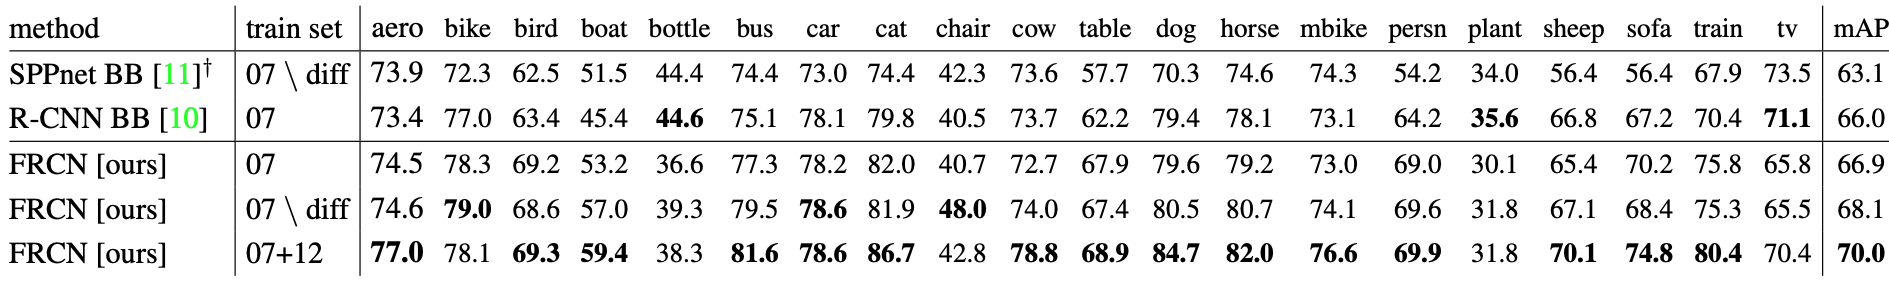
\includegraphics[width=15cm] {images/fast_rcnn_results_1}
            \caption{Kết quả của mô hình Fast R-CNN với các cấu hình khác nhau cùng các mô hình khác trên bộ dữ liệu VOC 2007 test}
            \label{fig:fast_rcnn_results_1}
        \end{figure}

        \noindent
        Tiếp theo, mô hình Fast R-CNN cũng có kết quả tốt trên bộ dữ liệu VOC 2010 test.
        Trong hình \ref{fig:fast_rcnn_results_2}, tác giả xét đến hai cấu hình của mô hình Fast R-CNN, các cấu hình này đều có kiến trúc như nhau (đều sử dụng mô hình VGG16 cho thành phần Feature extraction module) nhưng khác nhau về bộ dữ liệu train mà mỗi cấu hình sử dụng: \\
        - Cấu hình sử dụng bộ dữ liệu train là VOC12 trainval: ký hiệu là \textbf{12} \\
        - Cấu hình sử dụng bộ dữ liệu train là sự kết hợp giữa VOC07 trainval, VOC07 test và VOC12 trainval: ký hiệu là \textbf{07 ++ 12} \\
        Trong nhóm các mô hình so sánh, có kết quả của cấu hình tốt nhất của mô hình R-CNN là R-CNN BB.
        Ngoài ra còn có các mô hình BabyLearning (được train với bộ dữ liệu độc quyền) và mô hình SegDeepM (được train với bộ dữ liệu VOC 12 trainval bổ sung thêm các groundtruth segmentation). \\
        Kết quả của cấu hình \textbf{07 ++ 12} mô hình Fast R-CNN cho mAP cao hơn khoảng 2\% so với các cấu hình và mô hình khác.
        Tuy nhiên, vẫn tồn tại một số lớp đối tượng mà chỉ số AP của cấu hình này làm chưa tốt so với các cấu hình khác hay các mô hình khác như lớp \textit{bottle, plant, sheep, tv ...}.

        \begin{figure}[H]
            \centering
            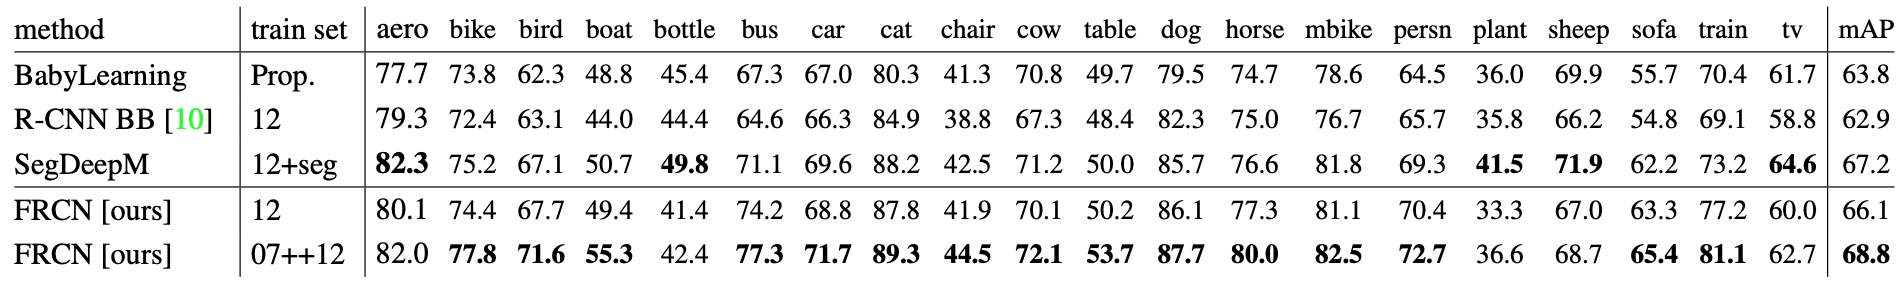
\includegraphics[width=15cm] {images/fast_rcnn_results_2}
            \caption{Kết quả của mô hình Fast R-CNN với các cấu hình khác nhau cùng các mô hình khác trên bộ dữ liệu VOC 2010 test}
            \label{fig:fast_rcnn_results_2}
        \end{figure}

        \noindent
        Đối với bộ dữ liệu VOC 2012 test, tác giả vẫn sử dụng hai cấu hình \textbf{12} và \textbf{07 ++ 12} của mô hình Fast R-CNN từ kết quả trên. Nhóm các mô hình so sánh gồm cấu hình R-CNN BB của mô hình R-CNN, mô hình BabyLearning (được train với bộ dữ liệu độc quyền) và mô hình NUS\_NIN\_c2000. \\
        Trong hình \ref{fig:fast_rcnn_results_3}, kết quả của cấu hình \textbf{07 ++ 12} mô hình Fast R-CNN cho mAP cao hơn khoảng 3-5\% so với các cấu hình và mô hình khác. \\
        Kết quả này vẫn tồn tại một số lớp đối tượng mà chỉ số AP của cấu hình này làm chưa tốt so với các cấu hình khác hay các mô hình khác như lớp \textit{bottle, plant}.

        \begin{figure}[H]
            \centering
            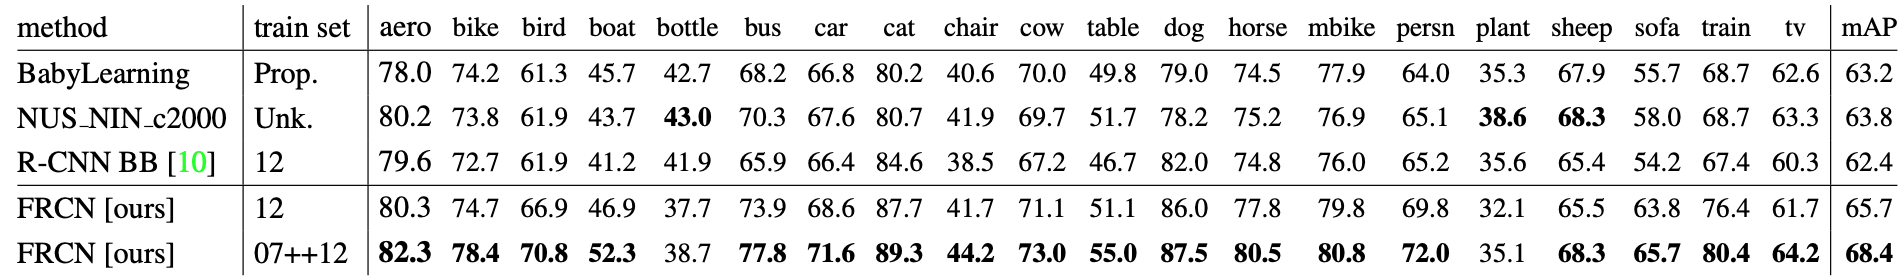
\includegraphics[width=15cm] {images/fast_rcnn_results_3}
            \caption{Kết quả của mô hình Fast R-CNN với các cấu hình khác nhau cùng các mô hình khác trên bộ dữ liệu VOC 2012 test}
            \label{fig:fast_rcnn_results_3}
        \end{figure}

        \noindent
        Cuối cùng, tác giả chia sẻ kết quả khi so sánh về mặt tốc độ trong quá trình train và quá trình test và đây là một trong số những thành quả chính. \\
        Trong hình \ref{fig:fast_rcnn_results_4}, tác giả so sánh tốc độ xử lý mỗi ảnh trong quá trình train và test giữa mô hình Fast R-CNN, R-CNN và SPPnet.
        Cụ thể hơn, trong quá trình train, thời gian train của mô hình Fast R-CNN giảm tới 8.8 lần so với mô hình R-CNN.
        Trong quá trình test, thời gian mà mô hình Fast R-CNN xử lý một ảnh nhanh hơn tới 146 (khi không sử dụng SVD) và tới 213 lần (khi sử dụng SVD) so với mô hình R-CNN.
        Không những thế, với việc cải thiện đáng kể tốc độ train và test, kết quả về độ chính xác của Fast R-CNN vẫn tốt hơn so với R-CNN khi so sánh trên chỉ số mAP.

        \begin{figure}[H]
            \centering
            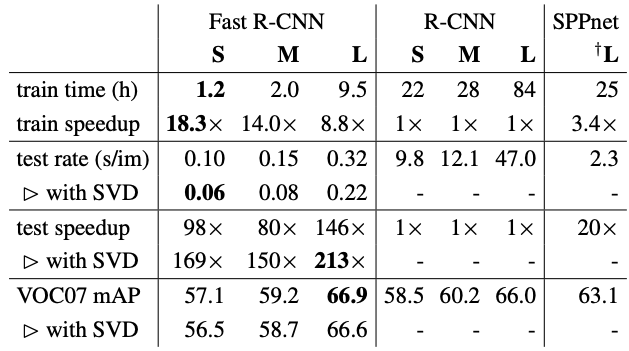
\includegraphics[width=10cm] {images/fast_rcnn_results_4}
            \caption{Kết quả so sánh về mặt tốc độ và độ chính xác giữa các cấu hình khác nhau của mô hình Fast R-CNN, R-CNN và SPPnet.}
            \label{fig:fast_rcnn_results_4}
        \end{figure}

        \noindent
        \textbf{\textit{Vấn đề tồn đọng của mô hình Fast R-CNN}} \\
        Những kết quả vượt bậc về mặt tốc độ của mô hình Fast R-CNN đã giải quyết được vấn đề tồn đọng của R-CNN trong khi vẫn duy trì được độ chính xác cao.
        Tuy nhiên, kiến trúc của mô hình Fast R-CNN vẫn phụ thuộc vào một thuật toán đề xuất khu vực như Selective Search và điều này tạo động lực để các nhà nghiên cứu xây dựng mô hình deep learning thay thế cho các thuật toán này.

    \subsubsection{Mô hình Faster R-CNN}
    
    \subsection{Các mô hình single-stage giải quyết bài toán Object Detection}
    \subsection{Mô hình SSD}

    \subsection{Nhóm các mô hình YOLO}

    \subsection{Mô hình RetinaNet}
    \subsubsection{Kiến trúc Feature Pyramid Network}
    - Nhắc thêm đến backbone ResNet
    \subsubsection{Hàm Focal loss}
}
    \objectdetection

    \newpage
    \def\objectdetectionhighres{
    \section{Các mô hình giải quyết bài toán object detection trong ảnh chất lượng cao}
    Bài toán object detection trong ảnh chất lượng cao là một chủ đề nhận được nhiều sự quan tâm trong thời gian vừa qua với nhiều nghiên cứu có giá trị tập trung để giải quyết hái vấn đề lớn là độ chính xác và tốc độ của mô hình.
    Các nghiên cứu này được chia làm hai trường phái: \\
    - Nhóm 1 bao gồm các giải pháp dựa trên ý tưởng chung là chia ảnh đầu vào có kích thước lớn thành dạng grid, sau đó thiết kế một thuật toán để giúp mô hình deep learning sử dụng các ảnh từ grid và tổng hợp các kết quả đầu ra lại trở thành một kết quả chung cho ảnh đầu vào có kích thước lớn.
    Các phương pháp trong nhóm này đạt độ chính xác tương đối cao do xử lý toàn bộ ảnh đầu vào và không bỏ đi khu vực nào trên ảnh, nhưng tốc độ lại không thực sự nhanh do phải xử lý một số lượng ảnh nhỏ từ grid rất lớn. \\
    - Nhóm 2 bao gồm các giải pháp dựa trên ý tưởng chung là thiết kế một mô hình hoặc một thuật toán riêng biệt xác định vị trí nào trên ảnh đầu vào có kích thước lớn là vị trí đáng chú ý và cần tập trung.
    Từ đó, loại bỏ đi các phần chứa ít thông tin trên ảnh đầu vào.
    Độ chính xác của các phương pháp trong nhóm này phụ thuộc nhiều vào mô hình hoặc thuật toán xác định vị trí đáng chú ý.
    Tuy nhiên, tốc độ của nhóm mô hình này lại rất tốt vì chúng đã bỏ qua phần lớn các khu vực trên ảnh đầu vào.

    \noindent
    Trong khuôn khổ nghiên cứu của luận văn, ta sẽ cùng tìm hiểu kỹ hơn về lý do tại sao bài toán object detection trong ảnh chất lượng cao lại là một bài toán khó trong \textbf{\textit{phần 3.1. Các thí nghiệm về tỷ lệ giữa kích thước của đối tượng trong ảnh và kích thước ảnh}}. Sau đó, ta bàn luận về một số phương pháp chuẩn bị dữ liệu tiêu biểu thuộc nhóm 2 qua các \textbf{\textit{phần 3.2. Phương pháp chuẩn bị dữ liệu SNIP, phần 3.3. Phương pháp chuẩn bị dữ liệu SNIPER, phần 3.4. Mô hình AutoFocus}}.

    \subsection{Các thí nghiệm về tỷ lệ giữa kích thước của đối tượng trong ảnh và kích thước ảnh}
    \def\highresexperiments{
    Trước khi bàn luận đến những mô hình giúp giải quyết bài toán object detection trong ảnh chất lượng cao, ta cần xem xét đến vai trò của tỷ lệ giữa kích thước của đối tượng trong ảnh và kích thước ảnh thông qua một số thí nghiệm.
    Cụ thể hơn, nhóm tác giả muốn đánh giá sự ảnh hưởng \textit{domain shift} lên kết quả của mô hình.
    \textit{Domain shift} được định nghĩa là sự thay đổi về tỷ lệ giữa kích thước của đối tượng trong ảnh và kích thước ảnh giữa tập dữ liệu train và tập dữ liệu test.
    \textit{Domain shift} rất phổ biến trong bài toán object detection, khi kích thước ảnh sử dụng trong quá trình train thường nhỏ (nhằm cải thiện tốc độ train mô hình) và kích thước ảnh sử dụng trong quá trình test thường lớn hơn (nhằm cải thiện độ chính xác của mô hình).
    Các thí nghiệm này được xây dựng và công bố kết quả bởi nhóm tác giả của mô hình SNIP \cite{singh2018analysis}.

    \noindent
    \textbf{\textit{Các thí nghiệm trong bài toán image classification}} \\
    Ba mô hình được sử dụng trong các thí nghiệm được thiết kế như sau: \\
    - Mô hình CNN-B: Đây là mô hình CNN sử dụng backbone ResNet-101 và đã được train với bộ dữ liệu ảnh có kích thước 224x224. \\
    - Mô hình CNN-S: Đây là mô hình CNN sử dụng backbone ResNet-101 và đã đã được thay đổi các tham số stride và kích thước của conv trong lớp đầu tiên đối với từng bộ dữ liệu ảnh có kích thước khác nhau khi train mô hình.
    Khi train với bộ dữ liệu ảnh có kích thước 48x48, tác giả dùng conv có kích thước 3x3 và stride bằng 1, khi train với bộ dữ liệu ảnh có kích thước 96x96, tác giả dùng conv có kích thước 5x5 và stride bằng 2. \\
    - Mô hình CNN-B-FT: Đây là mô hình CNN sử dụng backbone ResNet-101 và đã được train với bộ dữ liệu ảnh có kích thước 224x224 giống như CNN-B.
    Sau đó fine-tune lại với bộ dữ liệu ảnh có kích thước nhỏ hơn nhưng được upsample lên lại kích thước 224x224.

    \begin{figure}[H]
        \centering
        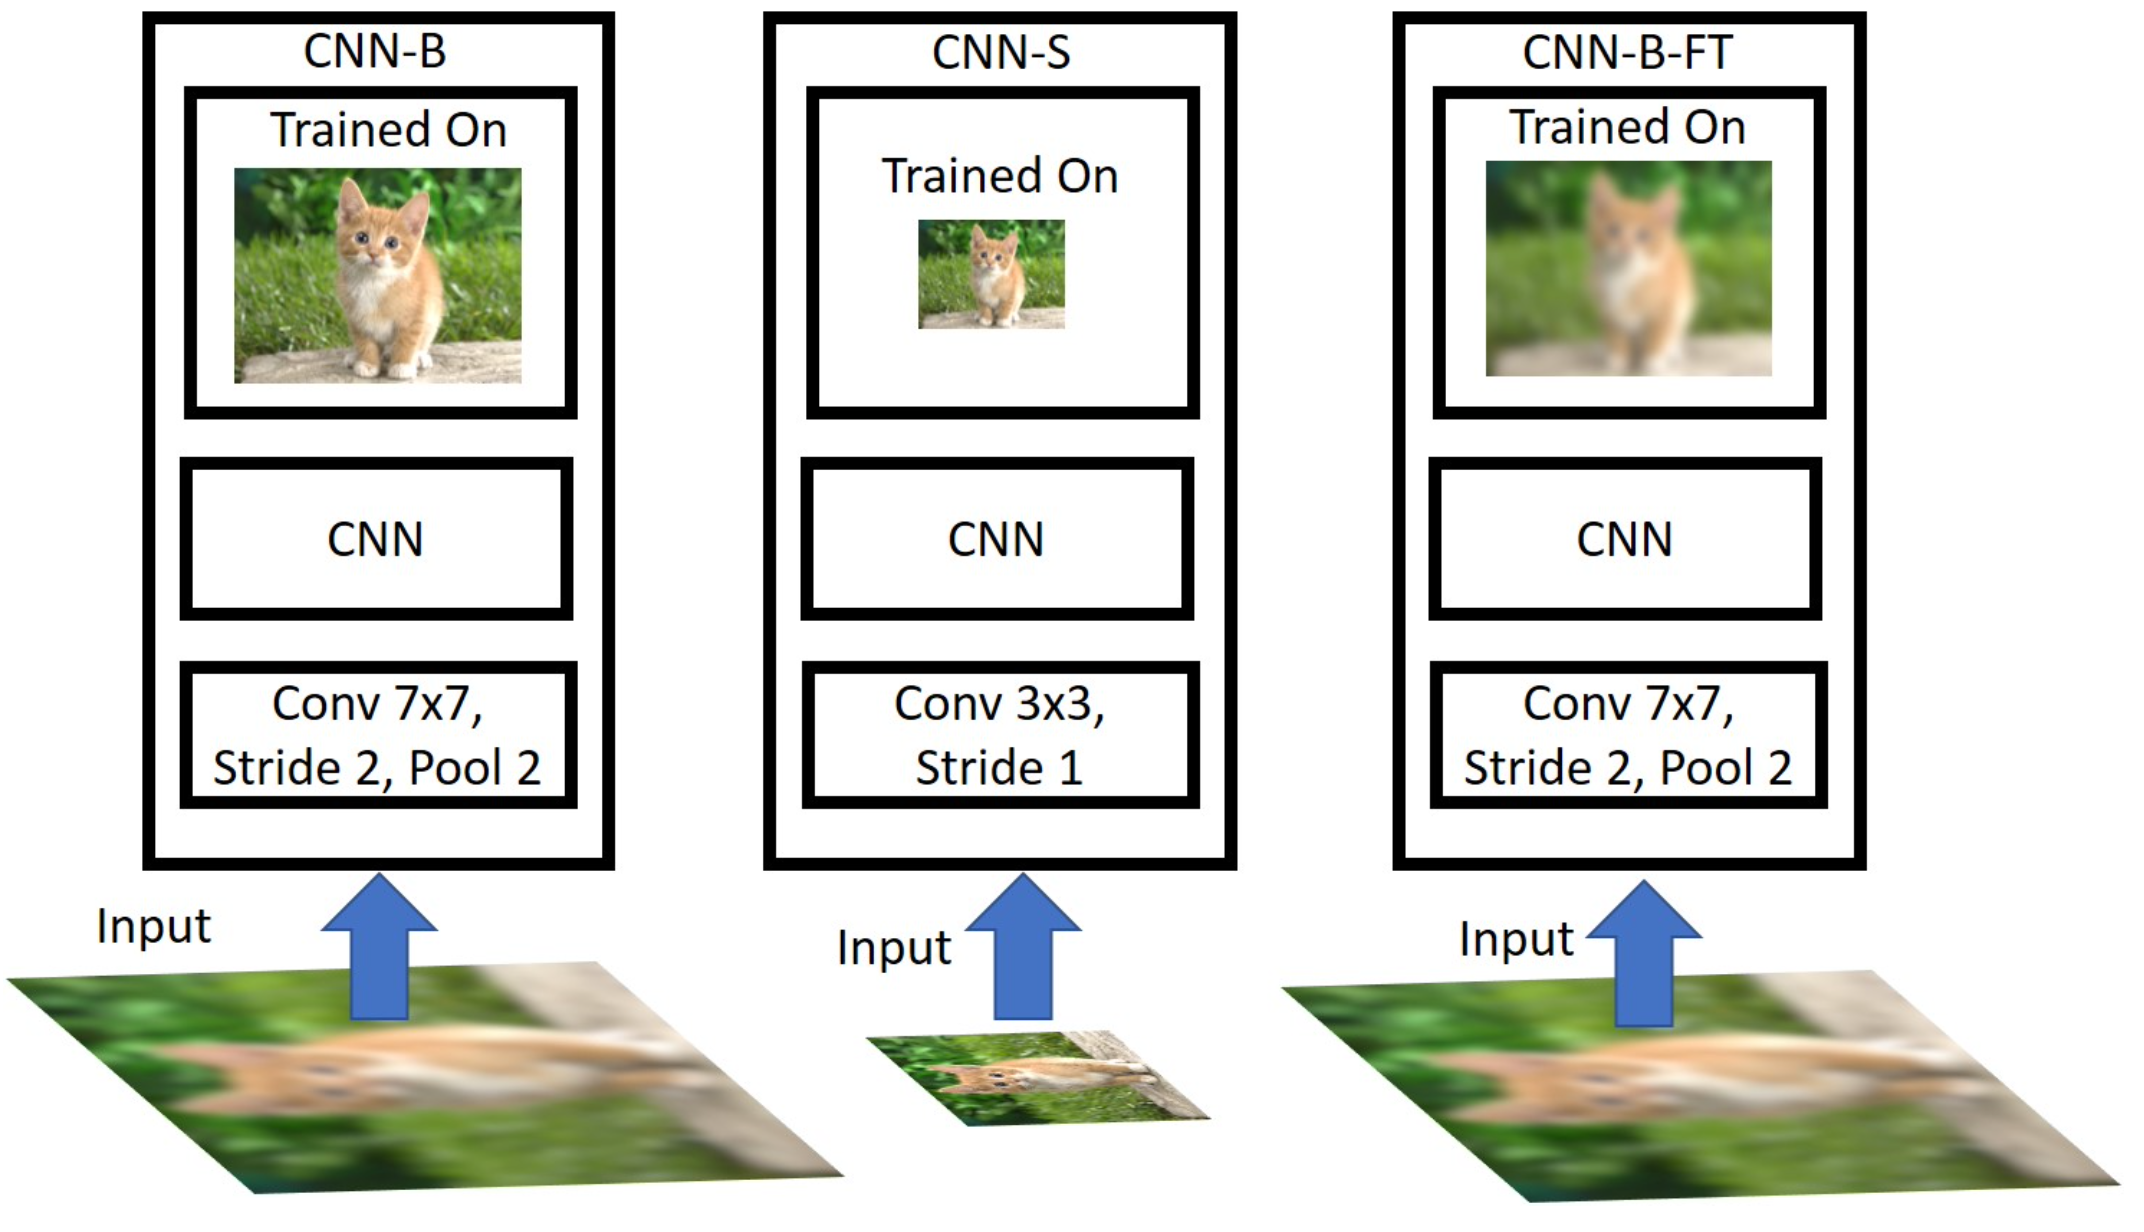
\includegraphics[width=12cm] {images/snip_models_to_exp.png}
        \caption{Ba mô hình được sử dụng trong các thí nghiệm (Nguồn: \cite{singh2018analysis})}
        \label{fig:snip_models_to_exp}
    \end{figure}

    \noindent 
    Nhóm tác giả thực hiện thí nghiệm đầu tiên là \textit{Thí nghiệm Naive Multi-Scale Inference}.
    Nhóm tác giả kiểm tra đánh giá mô hình CNN-B đơn giản với các bộ dữ liệu có kích thước ảnh khác nhau.
    Đầu tiên, nhóm tác giả thu nhỏ kích thước ảnh trong bộ dữ liệu ImageNet từ 224x224 xuống 48x48, 64x64, 80x80, 96x96, 128x128.
    Tiếp theo, nhóm tác giả tăng kích thước ảnh từ 48x48, 64x64, 80x80, 96x96, 128x128 lên lại 224x224.
    Cuối cùng, với các bộ dữ liệu mới nói trên, nhóm tác giả đưa vào mô hình CNN-B và quan sát kết quả.

    \begin{figure}[H]
        \centering
        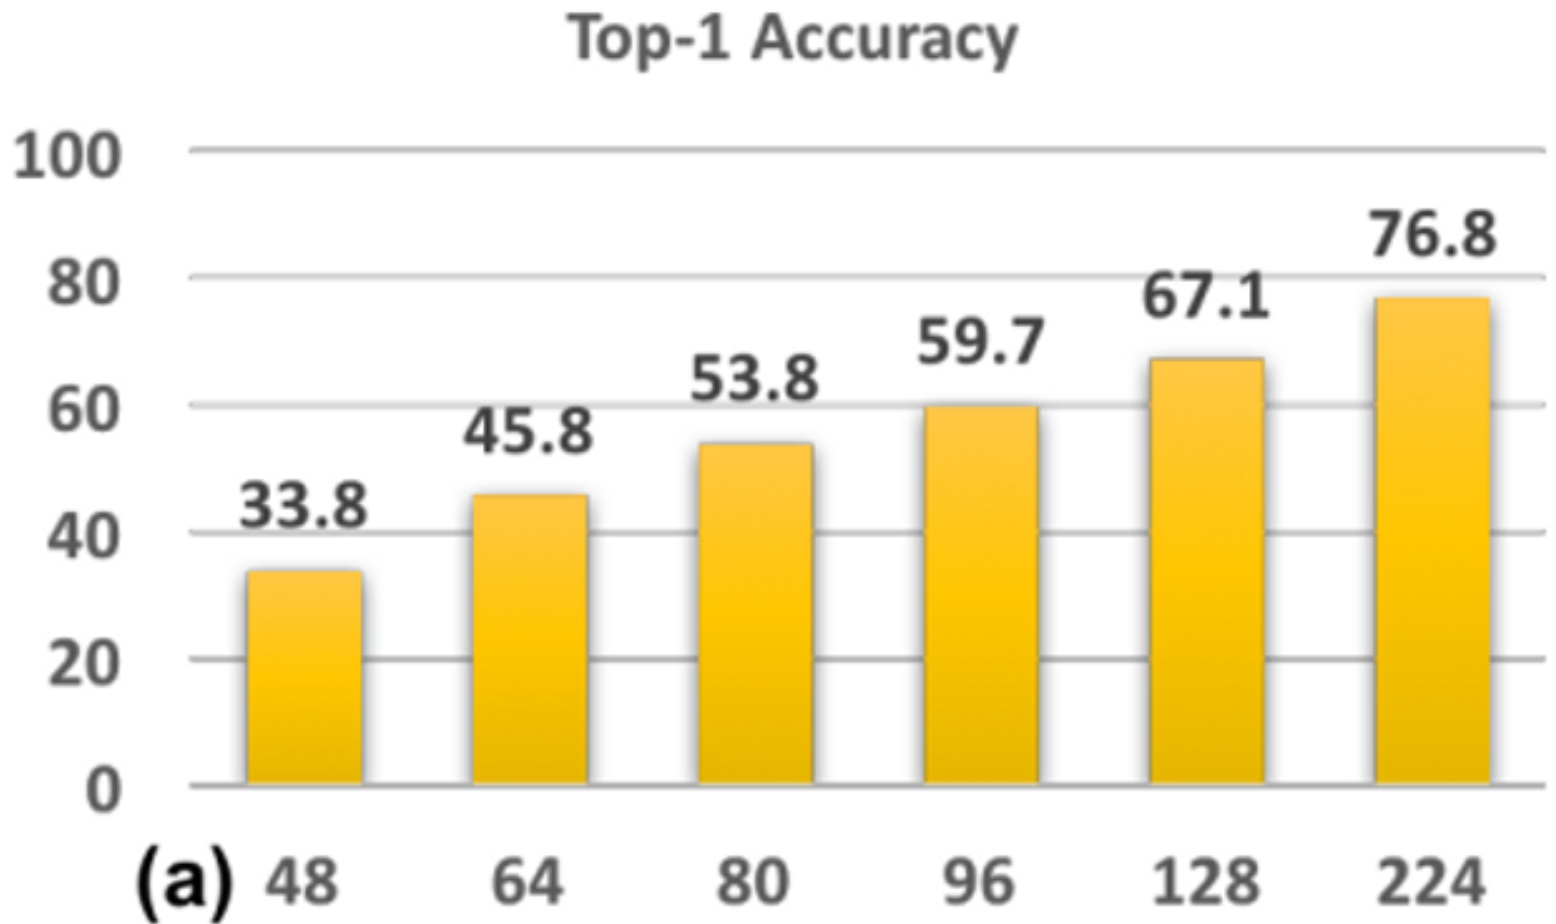
\includegraphics[width=9cm] {images/snip_naive_multi_scale_infer}
        \caption{Kết quả của thí nghiệm Naive Multi-Scale Inference (Nguồn: \cite{singh2018analysis})}
        \label{fig:snip_naive_multi_scale_infer}
    \end{figure}

    \noindent
    \textbf{Kết quả}:
    Ảnh sử dụng trong quá trình train và trong quá trình test càng khác nhau về kích thước, khả năng của mô hình càng giảm.
    Cụ thể hơn, kết quả về top-1 accuracy của mô hình CNN-B với các bộ dữ liệu được tăng kích thước từ 48x48, 64x64, 80x80, 96x96, 128x128 lần lượt là 33.8\%, 45.8\%, 53.8\%, 59.7\%, 67.1\%.
    Trong khi đối với bộ dữ liệu được giữ nguyên kích thước 224x224, mô hình CNN-B đạt kết quả 76.8\%. \\
    \textbf{Kết luận}:
    Đối với bài toán classification, việc test mô hình với các kích thước ảnh khác mà mô hình chưa được train sẽ gây ra kết quả suy giảm đáng kể.
    Sự chênh lệch càng lớn giữa kích thước ảnh train và kích thước ảnh test càng gây ra sự suy giảm kết quả đáng kể.

    \noindent
    Nhóm tác giả thực hiện thí nghiệm thứ hai là \textit{Thí nghiệm Resolution Specific Classifiers}.
    Trong thí nghiệm này, nhóm tác giả thay đổi một chút kiến trúc của mô hình CNN-S.
    Trong kiến trúc của mô hình CNN-B, lớp conv đầu tiên có kích thước stride = 2, và sau đó là lớp max pooling với stride = 2x2.
    Do đó, ngay từ các lớp đầu tiên, các mô hình trên xoá đi các thông tin của các đối tượng nhỏ trong ảnh.
    Từ quan sát trên, nhóm tác giả thay đổi kiến trúc và tạo ra mô hình CNN-S sao cho nó đạt được kết quả tốt nhất trên bộ CIFAR10 (đây là bộ dữ liệu với kích thước ảnh nhỏ).
    Sau đó, nhóm tác giả so sánh kiến trúc của mô hình CNN-S với mô hình CNN-B.

    \begin{figure}[H]
        \centering
        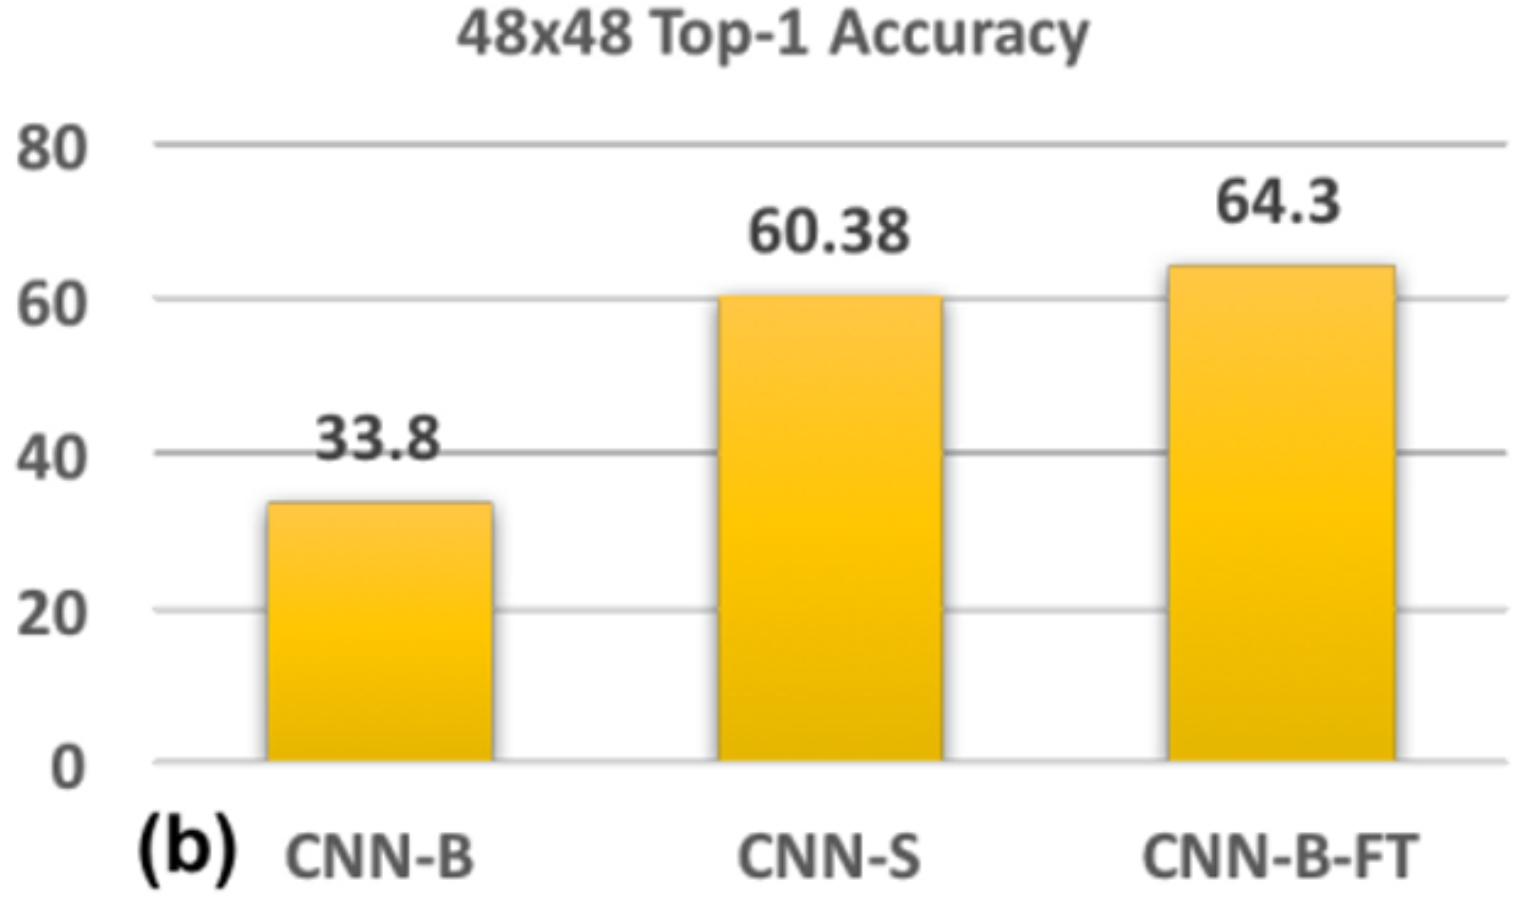
\includegraphics[width=9cm] {images/snip_res_spec_cls}
        \caption{Kết quả của thí nghiệm Resolution Specific Classifiers và Fine-tuning High-Resolution Classifiers trên bộ dữ liệu ảnh có kích thước 48x48 (Nguồn: \cite{singh2018analysis})}
        \label{fig:snip_res_spec_cls}
    \end{figure}

    \noindent
    \textbf{Kết quả}:
    Mô hình CNN-S đạt kết quả tốt hơn rất nhiều so với kết quả của mô hình CNN-B khi xử lý ảnh 48x48.
    Trong khi mô hình CNN-B đạt kết quả 33.8\%, mô hình CNN-S đạt kết quả 60.38\%. \\
    \textbf{Kết luận}:
    Việc thay đổi kiến trúc của mô hình sao cho phù hợp giúp cho mô hình học ảnh có resolution nhỏ tốt hơn.

    \noindent
    Nhóm tác giả thực hiện thí nghiệm cuối cùng trong phần này là \textit{Thí nghiệm Fine-tuning High-Resolution Classifiers}.
    Việc thiết kế và train mô hình (tương như như phương án của mô hình CNN-S trong thí nghiệm Resolution Specific Classifiers) với mỗi một bộ dữ liệu có kích thước ảnh khác nhau sẽ tốn quá nhiều công sức và tài nguyên tính toán.
    Từ đó, nhóm tác giả đưa ra một giải pháp đơn giản hơn đó là chiến lược xây dựng mô hình CNN-B-FT.

    \begin{figure}[H]
        \centering
        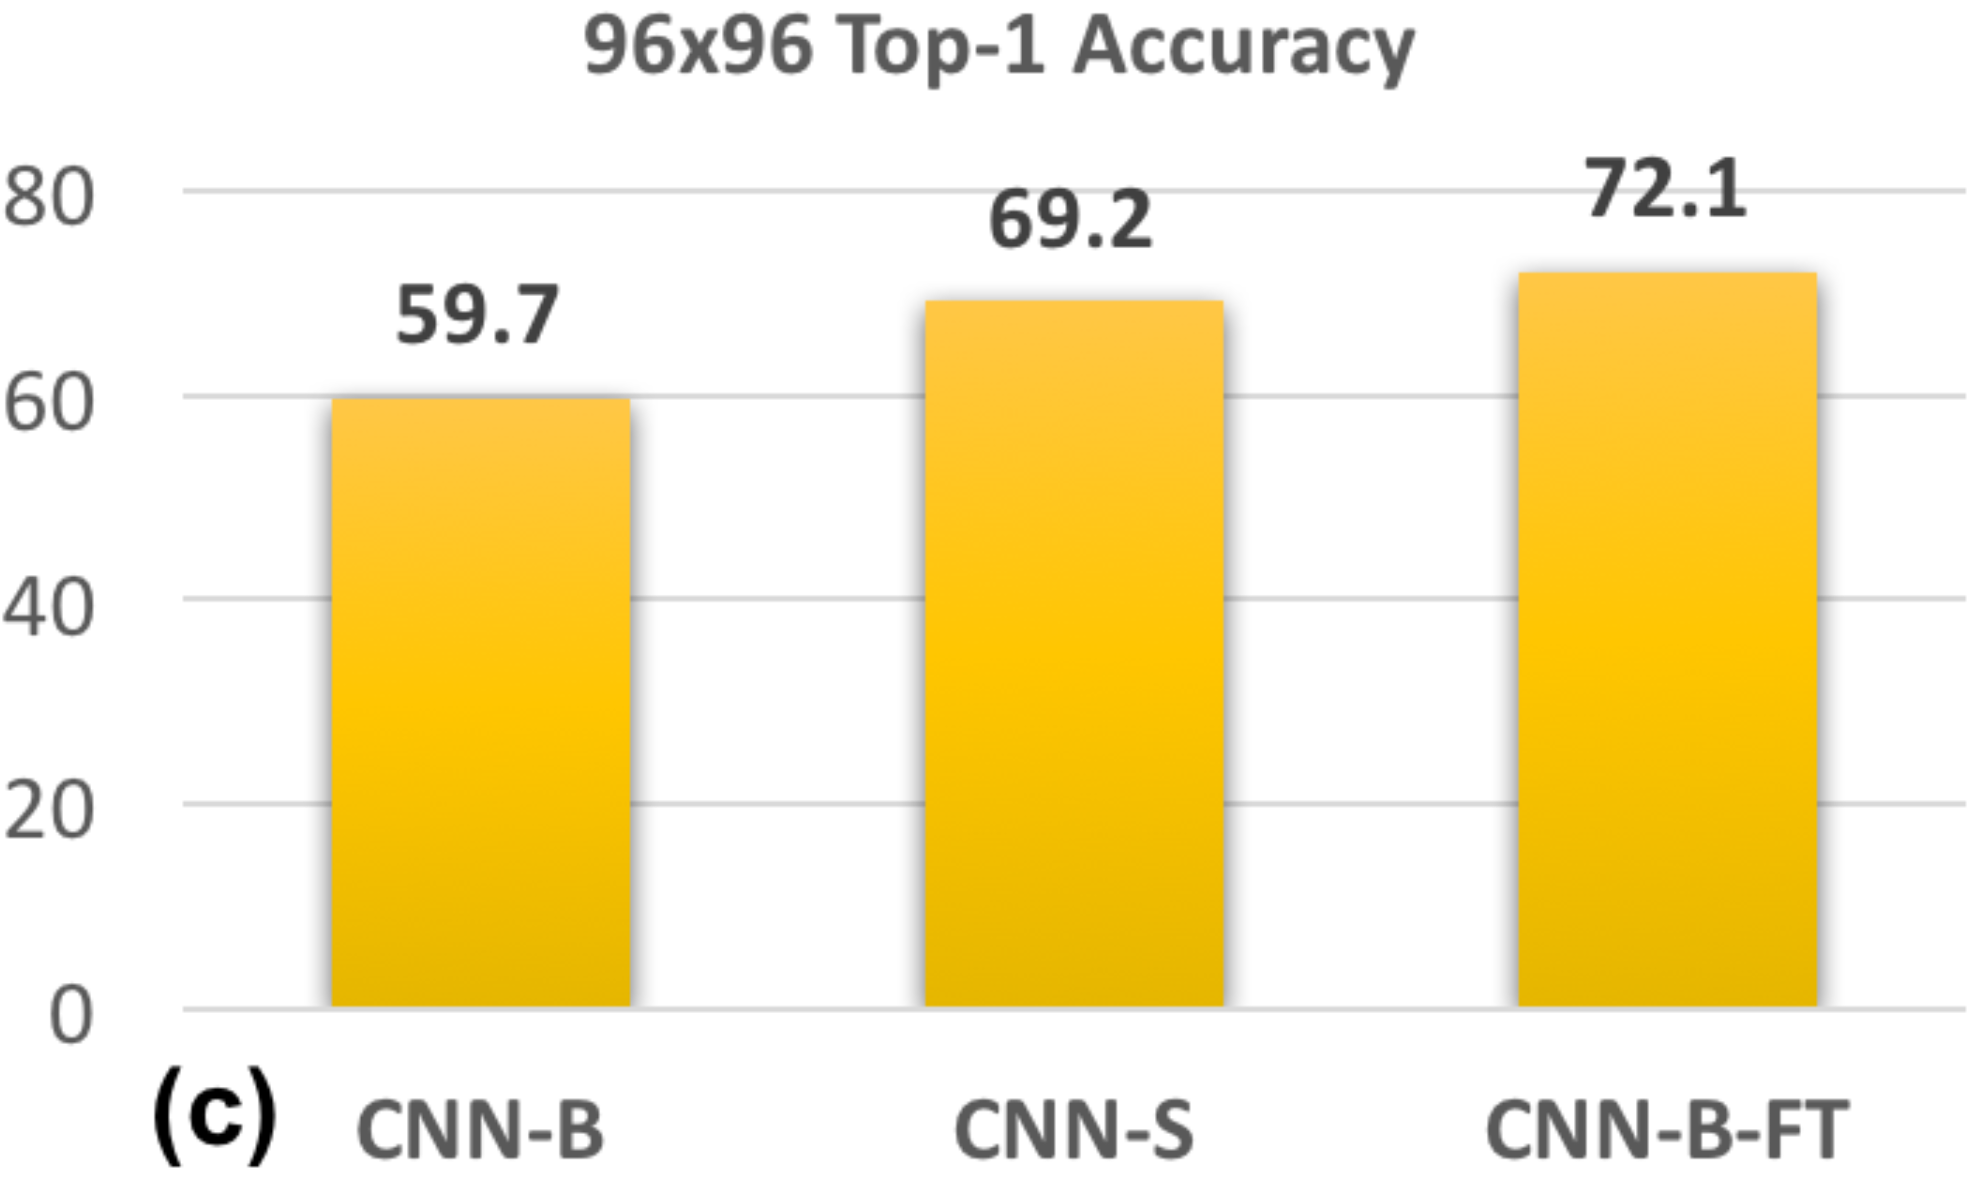
\includegraphics[width=9cm] {images/snip_res_spec_cls_96}
        \caption{Kết quả của thí nghiệm Resolution Specific Classifiers và Fine-tuning High-Resolution Classifiers trên bộ dữ liệu ảnh có kích thước 96x96 (Nguồn: \cite{singh2018analysis})}
        \label{fig:snip_res_spec_cls_96}
    \end{figure}

    \noindent
    \textbf{Kết quả}:
    Mô hình CNN-B-FT có kết quả tốt hơn so với kết quả của mô hình CNN-S. \\
    \textbf{Kết luận}:
    Thí nghiệm trên chứng minh rằng, các trọng số của mô hình CNN-B, được train từ bộ dữ liệu ảnh có kích thước lớn, hữu ích trong việc giải quyết bộ dữ liệu ảnh có kích thước nhỏ.
    Từ đó, thay vì giảm kích thước stride của lớp conv đi 2 lần (như trong kiến trúc của mô hình CNN-S), ta nên tăng kích thước của ảnh chất lượng thấp lên lần và fine-tune lại với mô hình đã được train với bộ dữ liệu ảnh có kích thước lớn.
    Hay nói cách khác, thay vì thay đổi kiến trúc của mô hình để xử lý riêng với bộ dữ liệu ảnh có kích thước nhỏ, ta nên tận dụng mô hình pretrained và fine-tune lại mô hình đó với bộ dữ liệu ảnh có kích thước mong muốn.

    \noindent
    \textbf{\textit{Các thí nghiệm trong bài toán object detection}} \\
    Hiệu năng giữa các mô hình bị ảnh hưởng bởi sự khác nhau về kích thước của ảnh trong bộ dữ liệu train và bộ dữ liệu test đã được nhóm tác giả chứng minh ở các thí nghiệm trên.
    Tuy nhiên, trong thực tế, không phải lúc nào ta cũng có thể train và test mô hình với bộ dữ liệu ảnh có cùng kích thước, đặc biệt đối với bài toán object detection.
    Lý do vì những vấn đề liên quan đến bộ nhớ của GPU cũng như là tốc độ train, do đó, thông thường kích thước ảnh trong bộ dữ liệu sử dụng trong quá trình train thường nhỏ hơn so với kích thước ảnh trong quá trình test.

    \noindent
    Trong các thí nghiệm ở phần này, nhóm tác giả sử dụng chung mô hình là Deformable - RFCN \cite{dai2017deformable}, train với những bộ dữ liệu khác nhau nhưng cùng test trên bộ dữ liệu có kích thước 1400x2000 nhằm mục đích đánh giá hiệu năng trong việc xác định các đối tượng nhỏ (kích thước nhỏ hơn 32x32).

    \noindent
    Nhóm tác giả thực hiện thí nghiệm đầu tiên là \textit{Thí nghiệm train các mô hình với kích thước ảnh khác nhau}.
    Trong thí nghiệm này, nhóm tác giả train mô hình với hai bộ dữ liệu lần lượt có kích thước ảnh là 800x1400 và 1400x2000 (tác giả lần lượt gọi là ${800}_{all}$ và ${1400}_{all}$).
    Và toàn bộ các đối tượng của cả hai bộ dữ liệu này đều được sử dụng để train. \\
    \textbf{Kết quả}:
    Hiển nhiên, ${1400}_{all}$ hoạt động tốt hơn so với ${800}_{all}$.
    Tuy nhiên, phần hơn của ${1400}_{all}$ là chưa đáng kể. \\
    \textbf{Kết luận}:
    Việc train ${1400}_{all}$ với ảnh có kích thước lớn hơn giúp các đối tượng nhỏ được tăng kích thước so với ${800}_{all}$, từ đó, các đối tượng này được train một cách dễ dàng hơn.
    Nhưng ở chiều ngược lại, những đối tượng trung bình và lớn trong ảnh cũng bị tăng kích thước theo khiến cho chúng trở nên quá lớn và trở nên khó khăn cho ${1400}_{all}$ có thể học một cách chính xác.
    Lượng dữ liệu khó học từ đối tượng trung bình và lớn này khiến cho ${1400}_{all}$ không thể vượt trội so với ${800}_{all}$.

    \begin{figure}[H]
        \centering
        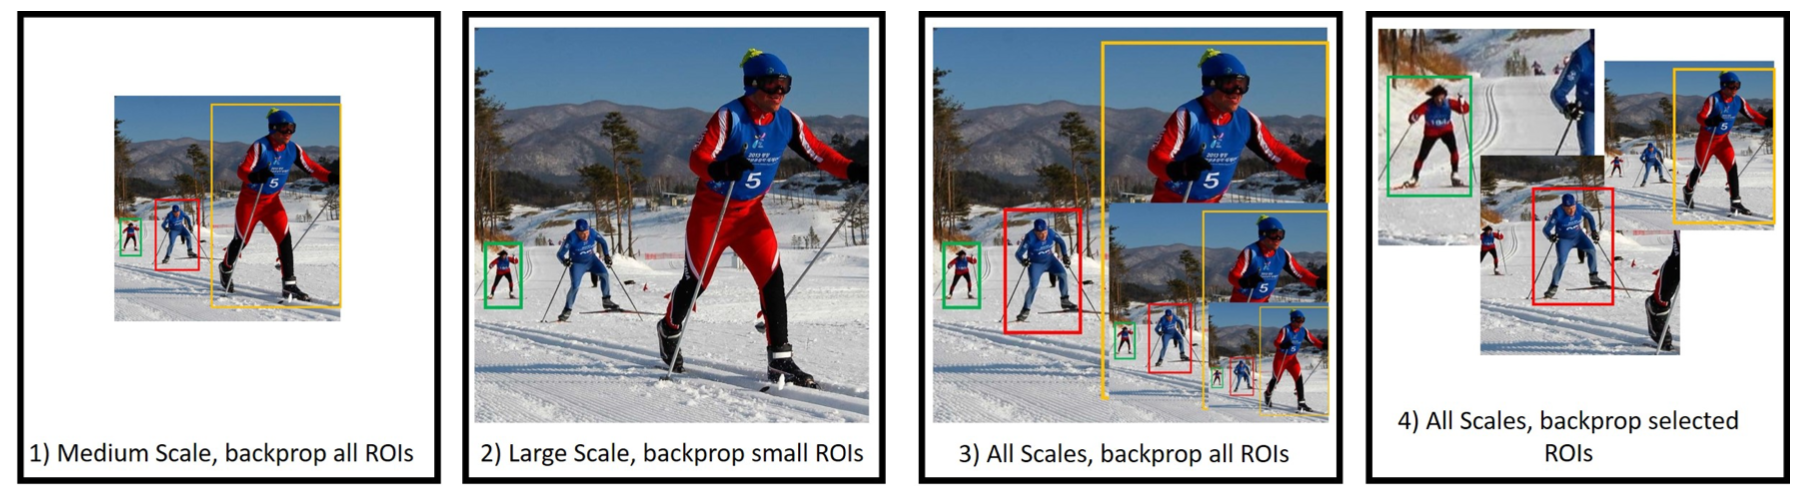
\includegraphics[width=15cm] {images/snip_model_compare}
        \caption{Các cách train mô hình khác nhau 1. ${800}_{all}$, 2. ${1400}_{<80px}$, 3. MST, 4. SNIP (Nguồn: \cite{singh2018analysis})}
        \label{fig:snip_model_compare}
    \end{figure}

    \noindent
    Tiếp theo, nhóm tác giả thực hiện \textit{Thí nghiệm train mô hình với các đối tượng có kích thước cụ thể}.
    Trong thí nghiệm này, nhóm tác giả vẫn train mô hình với bộ dữ liệu có kích thước 1400x2000.
    Tuy nhiên, nhóm tác giả loại bỏ hoàn toàn các đối tượng trung bình và lớn (các đối tượng có kích thước lớn hơn 80 trong ảnh gốc) và gọi là ${1400}_{<80px}$ \\
    \textbf{Kết quả}:
    Kết quả của ${1400}_{<80px}$ rất tệ so với kết quả của ${800}_{all}$ và ${1400}_{all}$. \\
    \textbf{Kết luận}:
    Việc loại bỏ hoàn toàn các đối tượng trung bình và lớn khiến cho lượng dữ liệu mà ${1400}_{<80px}$ được học giảm đi rất nhiều so với các mô hình trên (giảm khoảng 30\% lượng biến thể của đối tượng).
    Từ đó, kết quả của ${1400}_{<80px}$ bị ảnh hưởng nghiêm trọng.
    Chúng ta cũng có thể rút ra được một kết luận là, cho dù các ${1400}_{all}$ và ${800}_{all}$ không hoàn toàn học được các đối tượng trung bình và lớn nhưng lượng dữ liệu từ các đối tượng này vẫn đóng vai trò quan trọng trong việc giúp các mô hình xác định các đối tượng nhỏ.

    \begin{figure}[H]
        \centering
        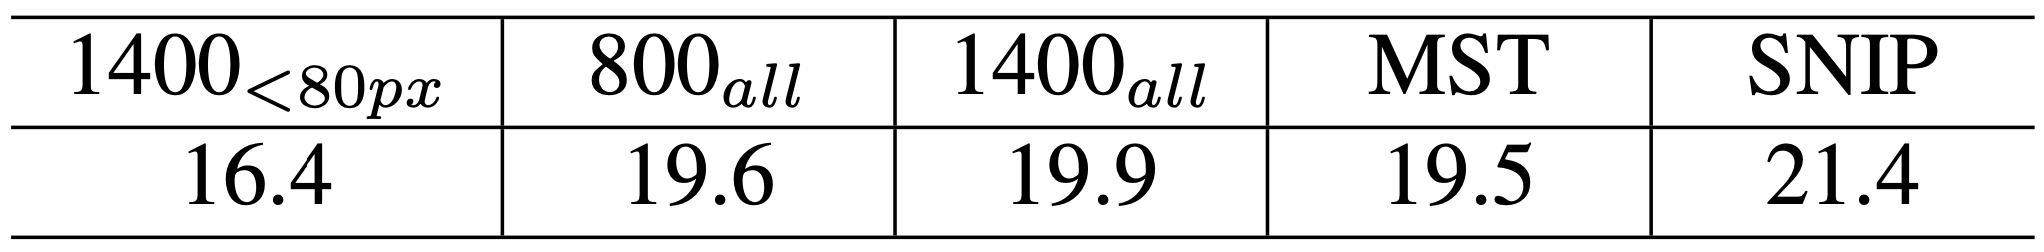
\includegraphics[width=13cm] {images/snip_results_1}
        \caption{So sánh kết quả trên chỉ số mAP của các mô hình ${1400}_{<80px}$, ${800}_{all}$, ${1400}_{all}$, MST và SNIP trên các đối tượng có kích thước nhỏ (nhỏ hơn 32x32) (Nguồn: \cite{singh2018analysis})}
        \label{fig:snip_results_1}
    \end{figure}

    \noindent
    Cuối cùng, nhóm tác giả thực hiện \textit{Thí nghiệm train với bộ dữ liệu ảnh có các kích thước khác nhau}.
    Nhóm tác giả train mô hình với bộ dữ liệu ảnh có các kích thước khác nhau được lựa chọn ngẫu nhiên trong suốt quá trình train (Multi-Scale Training) và gọi đó là MST.
    Thí nghiệm này giúp mô hình có thể được học các kích thước khác nhau với mỗi đối tượng trong bộ dữ liệu. \\
    \textbf{Kết quả}:
    Kết quả của MST xấp xỉ so với kết quả của ${800}_{all}$. \\
    \textbf{Kết luận}:
    Việc chuẩn bị dữ liệu ảnh có các kích thước khác nhau như MST khiến mô hình gặp khó khăn trong việc học các đối tượng rất lớn hoặc rất nhỏ.
    Điều này phần nào đó tương tự với hiện tượng mà ${1400}_{all}$ gặp phải.
}
    \highresexperiments

    \subsection{Phương pháp chuẩn bị dữ liệu SNIP}
    \def\snip{
    Từ những thí nghiệm trong \textit{phần 3.1}, nhóm tác giả đã đưa ra đề xuất phương pháp chuẩn bị dữ liệu Scale Normalization for Image Pyramids (gọi tắt là SNIP) \cite{singh2018analysis}.
    Phương pháp SNIP hướng đến việc sử dụng tối đa sự đa dạng trong biến thể của đối tượng trong bộ dữ liệu trong khi có thể thu hẹp được sự biến động trong kích thước của các đối tượng.
    Từ đó, mô hình sẽ có nhiều dữ liệu nhất có thể và cũng sẽ có kích thước đối tượng phù hợp nhất để học.
    Ý tưởng chung của SNIP dựa trên \textit{image pyramid} đã được nhắc đến trong phần \textit{phần 2.2. Kiến trúc Feature Pyramid Networks}.

    \noindent
    \textbf{\textit{Ý tưởng của phương pháp chuẩn bị dữ liệu SNIP}} \\
    Một điểm yếu của việc chuẩn bị dữ liệu MST ở thí nghiệm \textit{phần 3.1} là việc một ảnh bất kỳ được train với nhiều kích thước khác nhau khiến cho khi ảnh đó ở kích thước lớn (1400x2000) thì các đối tượng lớn sẽ trở nên khó khăn cho mô hình.
    Điều này diễn ra tương tự đối với các đối tượng nhỏ khi ảnh đó ở kích thước nhỏ (480x800).

    \begin{figure}[H]
        \centering
        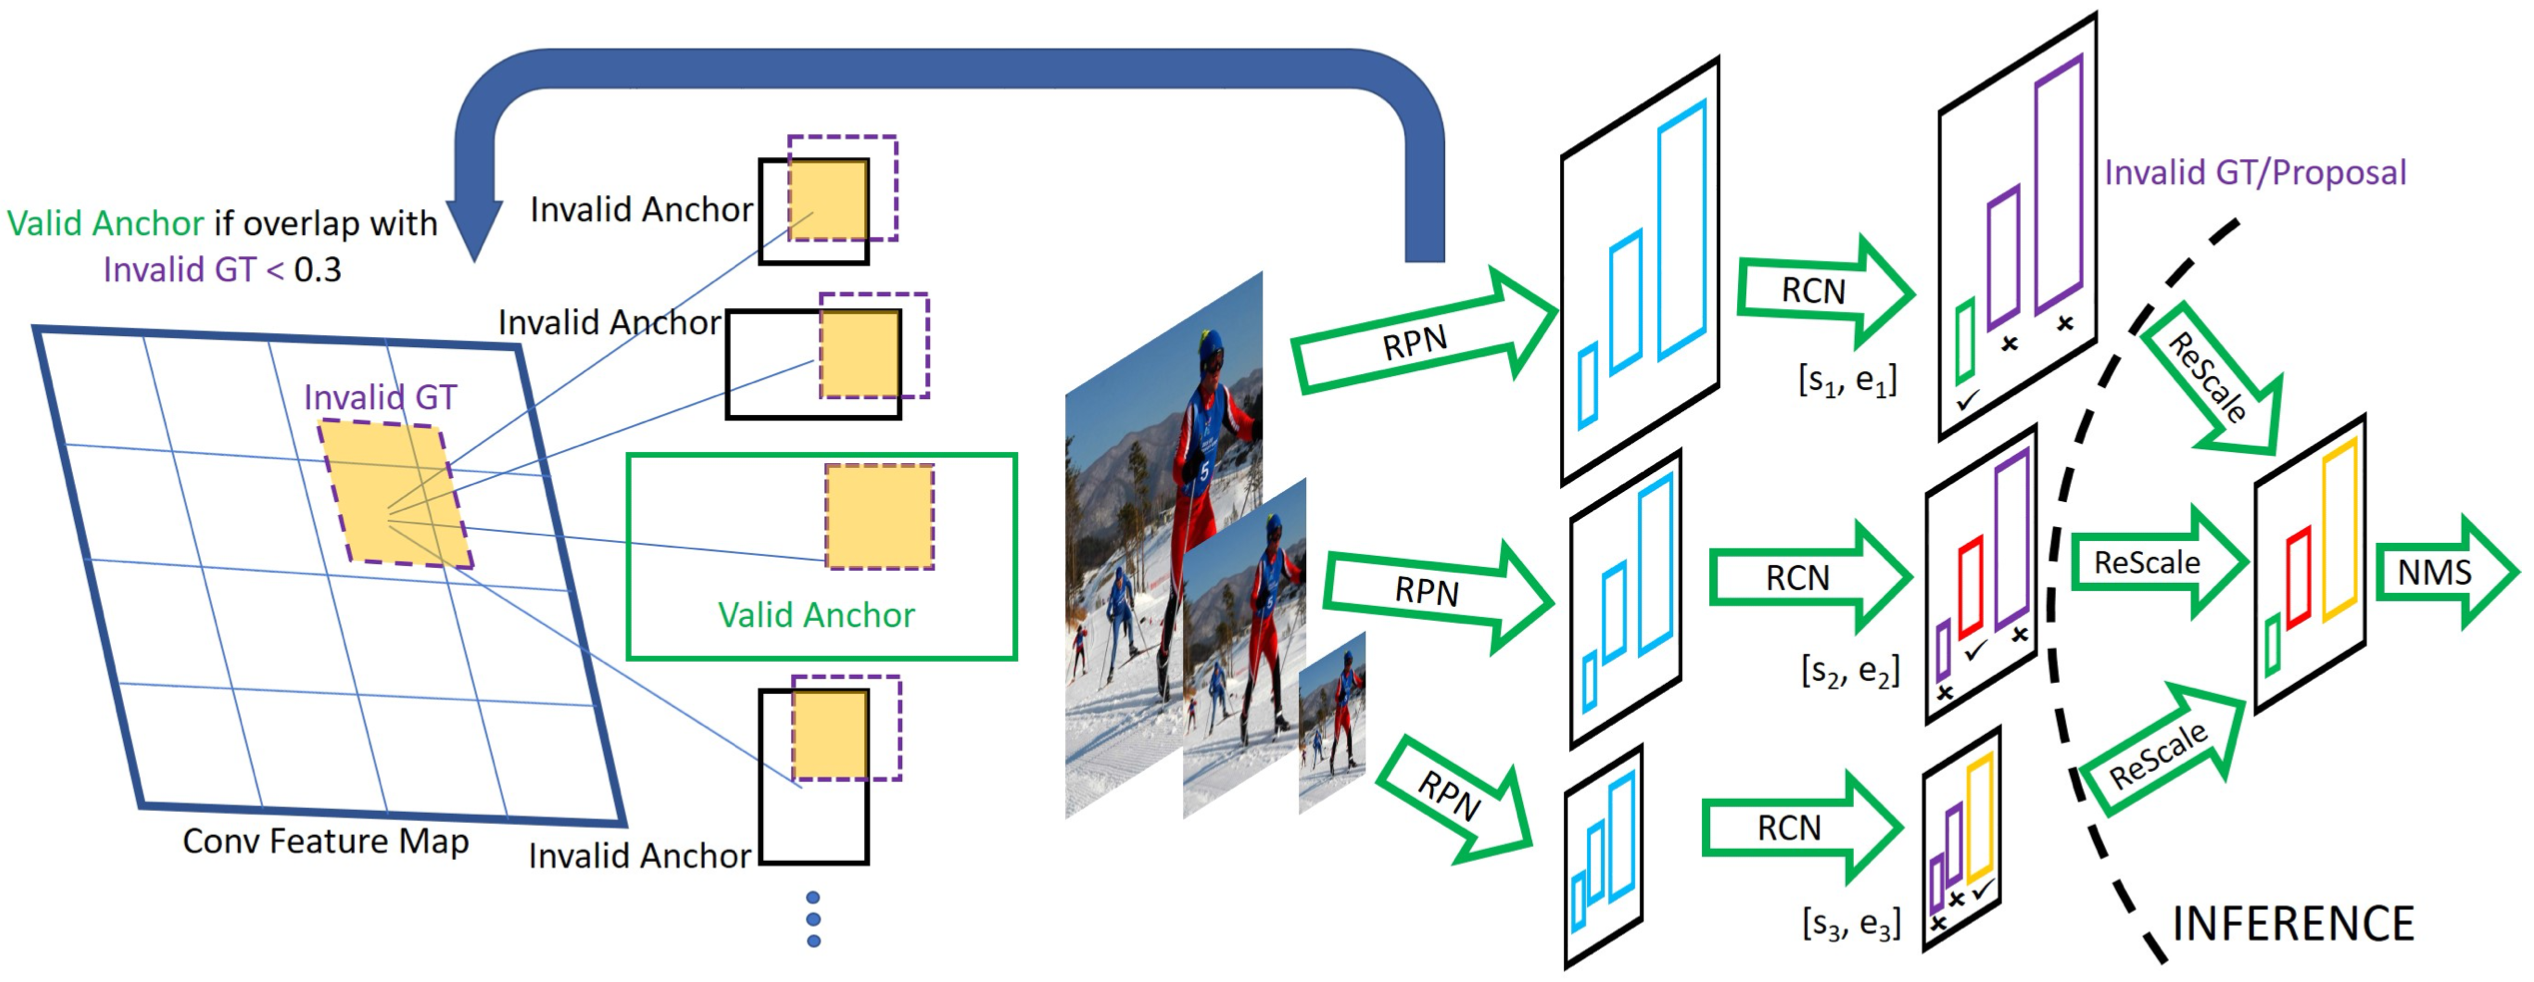
\includegraphics[width=16cm] {images/snip_model}
        \caption{Chi tiết kiến trúc phương pháp chuẩn bị dữ liệu SNIP trong quá trình train và test (Nguồn: \cite{singh2018analysis})}
        \label{fig:snip_model}
    \end{figure}

    \noindent
    phương pháp chuẩn bị dữ liệu SNIP được coi là một phiên bản nâng cấp hơn của MST.
    Ý tưởng chính của SNIP là trong quá trình train, các đối tượng có kích thước tương đồng với bộ dữ liệu pretrained của mô hình (thông thường là 224x224) sẽ được sử dụng để train và loại bỏ các đối tượng, mà sau khi thay đổi kích thước ảnh, trở nên quá lớn hoặc quá nhỏ.

    \noindent
    \textbf{\textit{Kết quả của mô hình khi sử dụng phương pháp chuẩn bị dữ liệu SNIP}} \\
    Kết quả của mô hình khi sử dụng phương pháp chuẩn bị dữ liệu SNIP so sánh với các thí nghiệm khác trong \textit{phần 3.1} được thể hiện ở hình \ref{fig:snip_results_1}.
    Việc sử dụng SNIP giúp mô hình đạt độ chính xác cao hơn so với các mô hình sử dụng các phương pháp chuẩn bị dữ liệu khác.

    \noindent
    Nhóm tác giả cũng so sánh kết kết quả của các mô hình sử dụng và không sử dụng phương pháp chuẩn bị dữ liệu SNIP cùng các kiến trúc backbone khác nhau.
    Các mô hình sử dụng trong thí nghiệm là D-RFCN \cite{}, Mask-RCNN \cite{}, G-RMI \cite{}, Faster-RCNN \cite{}.
    Kỹ thuật được bổ sung trong một số cấu hình là RCN \cite{}.
    Các cấu hình sử dụng phương pháp chuẩn bị dữ liệu SNIP có ký hiệu \textit{+ SNIP}.
    Chi tiết các backbone sử dụng trong mỗi cấu hình được chú thích ở cột \textit{Backbone}.
    
    \begin{figure}[H]
        \centering
        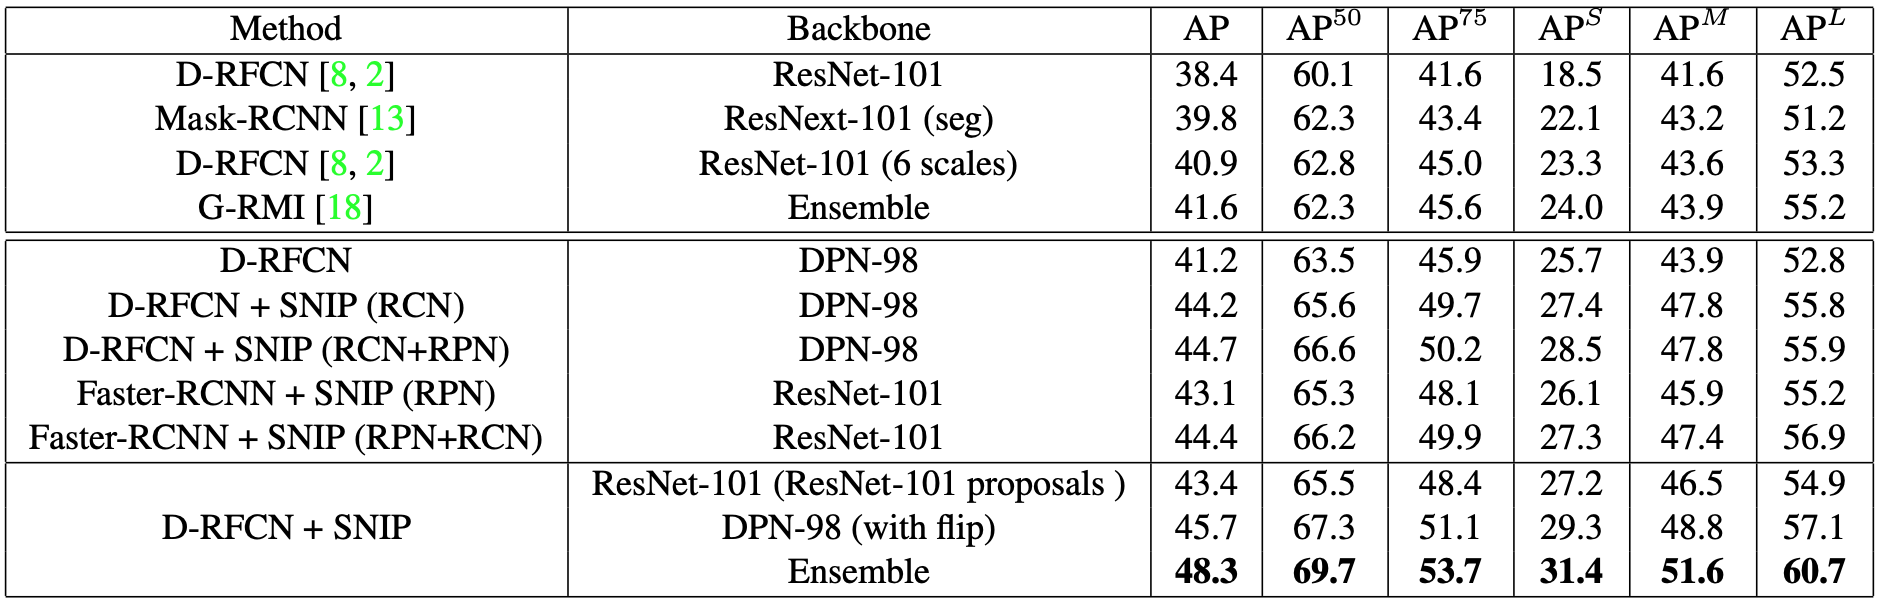
\includegraphics[width=16cm] {images/snip_results_2}
        \caption{Kết quả của các mô hình sử dụng và không sử dụng phương pháp chuẩn bị dữ liệu SNIP (Nguồn: \cite{singh2018analysis})}
        \label{fig:snip_results_2}
    \end{figure}

    \noindent
    Kết quả của mô hình D-RFCN sử dụng SNIP và backbone Ensemble đạt chỉ số cao hơn khá nhiều so với các cấu hình khác.
    Ngoài ra, các cấu hình sử dụng SNIP cũng đạt chỉ số cao hơn các cấu hình không sử dụng SNIP.
    Điều này chứng minh được vai trò của phương pháp chuẩn bị dữ liệu SNIP đối với các mô hình object detection.

    \noindent
    \textbf{\textit{Vấn đề tồn đọng của phương pháp chuẩn bị dữ liệu SNIP}} \\
    Tuy rằng đã có những cải thiện trong kết quả của các mô hình sử dụng phương pháp chuẩn bị dữ liệu SNIP, nhưng nhóm tác giả vẫn nêu ra những vấn đề tồn đọng là lãng phí chi phí tính toán trong quá trình train.
    Cụ thể, những đối tượng có kích thước lớn và bị loại bỏ trong quá trình train, nhưng các lớp Conv \index{lớp Conv} vẫn phải tính toán trên các phần này dẫn đến sự lãng phí tài nguyên tính toán.
}
    \snip

    \subsection{Phương pháp chuẩn bị dữ liệu SNIPER}
    \def\sniper{
    Xuất phát từ những vấn đề tồn đọng của phương pháp SNIP, nhóm tác giả \cite{singh2018sniper} đã đề xuất phương pháp chuẩn bị dữ liệu Scale Normalization for Image Pyramids with Efficient Resampling (gọi tắt là SNIPER \index{SNIPER}).
    Phương pháp chuẩn bị dữ liệu SNIPER \index{SNIPER} hướng đến việc giảm thiểu đến tối đa khối lượng tính toán dư thừa từ đó tăng tốc được quá trình huấn luyện mô hình.
    Nhóm tác giả đã thành công trong việc duy trì được kết quả mà SNIP đạt được trong khi SNIPER \index{SNIPER} chỉ cần xử lý số lượng pixels \index{pixels} ảnh bằng một phần ba số lượng mà SNIP phải xử lý.
    Điều này giúp việc huấn luyện bằng phương pháp SNIPER \index{SNIPER} tiết kiệm bộ nhớ hơn và có thể sử dụng được batch size lớn hơn trong quá trình huấn luyện.
    Mô hình object detection mà nhóm tác giả sử dụng để làm các thí nghiệm với SNIPER \index{SNIPER} là mô hình Faster R-CNN \cite{ren2015faster}.

    \noindent
    \textbf{\textit{Ý tưởng của phương pháp chuẩn bị dữ liệu SNIPER \index{SNIPER}}} \\
    Nhằm tối ưu hoá khối lượng tính toán trong quá trình huấn luyện, thay vì việc thay đổi kích thước của ảnh và chọn ra những object có kích thước phù hợp trong quá trình huấn luyện, phương pháp SNIPER \index{SNIPER} cung cấp một cơ chế tiền xử lý dữ liệu.
    Từ bộ dữ liệu gốc ban đầu, các thuật toán của SNIPER \index{SNIPER} xử lý và tạo ra bộ dữ liệu mới với các ảnh trong bộ dữ liệu được gọi là các Chip.

    \noindent
    \textbf{\textit{Định nghĩa Chip và phương pháp sinh ra Chip bằng phương pháp chuẩn bị dữ liệu SNIPER \index{SNIPER}}} \\
    Chip trong SNIPER \index{SNIPER} có thể được hiểu là một phần của bức ảnh và đây cũng là đơn vị dữ liệu sử dụng trong quá trình huấn luyện mô hình.
    Các bước sinh ra bộ Chip trong thuật toán SNIPER \index{SNIPER} như sau: \\
    - \textit{Bước 1}: Nhóm tác giả định nghĩa một danh sách các kích thước ảnh {${s}_{1}$, ${s}_{2}$, ..., ${s}_{i}$, ..., ${s}_{n}$}. \\
    - \textit{Bước 2}: SNIPER \index{SNIPER} thay đổi kích thước của từng ảnh gốc ban đầu về từng kích ${s}_{i}$ trong danh sách trên.
    Ta thu được một bộ dữ liệu ảnh mới, trong đó, mỗi ảnh trong bộ dữ liệu ảnh ban đầu tương ứng với n ảnh với các kích thước khác nhau trong bộ dữ liệu ảnh mới. \\
    - \textit{Bước 3}: Trên mỗi ảnh trong bộ dữ liệu ảnh mới, SNIPER \index{SNIPER} đặt các ô vuông có kích thước \textit{KxK} sao cho tâm của các ô vuông này cách đều nhau một khoảng \textit{d} pixels \index{pixels}. \\
    - \textit{Bước 4}: SNIPER \index{SNIPER} cắt ảnh theo các ô vuông đã đặt từ bước 3 để tạo thành các Chip. Danh sách các Chip này sẽ được lựa chọn và xử lý ở các thuật toán tiếp theo.

    \noindent
    \textbf{\textit{Phương pháp lựa chọn các positive Chips}} \\
    Từ danh sách các Chip đã được tạo ra bởi thuật toán trên, nhóm tác giả thực hiện thuật toán lựa chọn các positive Chips.
    positive Chip ở đây được hiểu là các Chip chứa các groundtruth \index{groundtruth} bounding box \index{bounding box} của object mà mô hình cần học.
    Các bước lựa chọn ra positive Chip trong phương pháp SNIPER \index{SNIPER} như sau: \\
    - \textit{Bước 1}: Nhóm tác giả định nghĩa một danh sách các khoảng kích thước bounding box \index{bounding box} phù hợp tương ứng với mỗi kích thước ảnh {${s}_{1}$, ..., ${s}_{n}$}.
    Cụ thể, với kích thước ảnh ${s}_{i}$, ta định nghĩa khoảng kích thước bounding box \index{bounding box} phù hợp ${R}^{i} = [{r}_{min}^{i}, {r}_{max}^{i}]$. \\
    - \textit{Bước 2}: SNIPER \index{SNIPER} kiểm tra từng bounding box \index{bounding box} trong từng Chip trên từng kích thước ảnh.
    Những bounding box \index{bounding box} có kích thước nằm trong khoảng kích thước phù hợp ${R}^{i}$ được thêm vào danh sách các bounding box \index{bounding box} hợp lệ ${G}^{i}$. \\
    - \textit{Bước 3}: SNIPER \index{SNIPER} lựa chọn các Chip từ danh sách các Chip ở thuật toán trên sao cho số lượng bounding box \index{bounding box} hợp lệ và nằm hoàn toàn trong một Chip là nhiều nhất.
    Danh sách các positive Chips trên mỗi ảnh trong cùng một kích thước được gọi là ${C}_{pos}^{i}$.

    \begin{figure}[H]
        \centering
        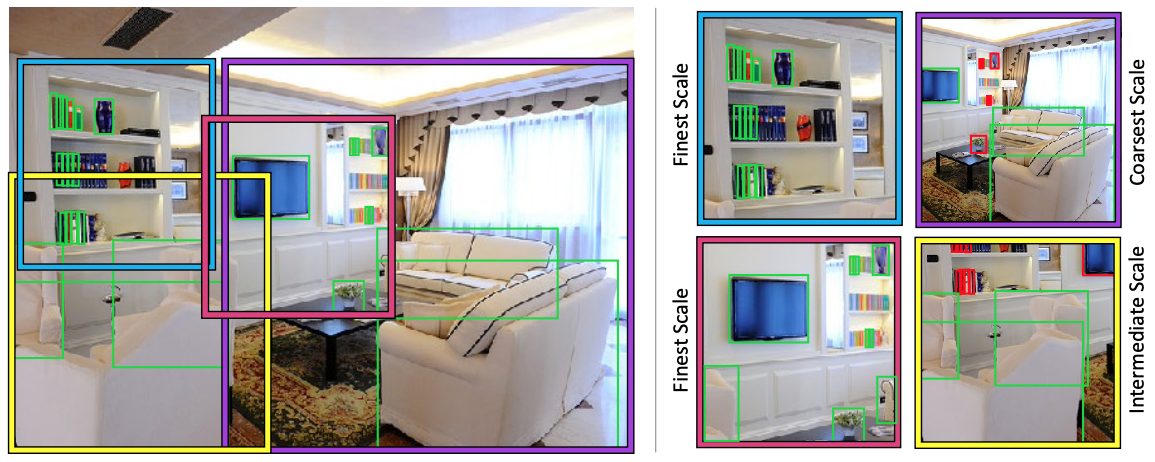
\includegraphics[width=13cm] {images/sniper_pos_chip}
        \caption{Kết quả thuật toán lựa chọn các positive chips (Nguồn: \cite{singh2018sniper})}
        \label{fig:sniper_pos_chip}
    \end{figure}

    \noindent
    Một groundtruth \index{groundtruth} bounding box \index{bounding box} bất kỳ sẽ luôn có một Chip nào đó chứa nó và có thể xuất hiện ở nhiều hơn một Chip trong cùng một kích thước ảnh hoặc trong nhiều kích thước ảnh khác nhau.
    Các groundtruth \index{groundtruth} bounding box \index{bounding box} không nằm hoàn toàn trong một chip sẽ bị cắt.
    Phần cắt nếu thoả mãn khoảng kích thước phù hợp sẽ được coi là hợp lệ, phần cắt nếu không thoả mãn khoảng kích thước phù hợp sẽ được coi là vi phạm nhưng vẫn được sử dụng để gán label cho các khu vực được đề xuất bởi mô hình RPN. \\
    Mỗi groundtruth \index{groundtruth} bounding box \index{bounding box} tìm được kích thước Chip phù hợp để học, và hơn nữa kích thước của mỗi Chip nhỏ hơn rất nhiều so với mỗi kích thước ảnh tương ứng của Chip đó.
    Điều này mang lại sự tiết kiệm trong cả nguồn bộ nhớ lẫn tốc độ tính toán. \\
    Trong hình \ref{fig:sniper_pos_chip}, từ ảnh và các groundtruth \index{groundtruth} bounding box \index{bounding box} ban đầu (ảnh bên phải), thuật toán của SNIPER \index{SNIPER} đã cắt ra được các Chip (ảnh bên trái), mỗi Chip sẽ tương ứng chứa các groundtruth \index{groundtruth} bounding box \index{bounding box} hợp lệ (các bounding box \index{bounding box} màu xanh) và các groundtruth \index{groundtruth} bounding box \index{bounding box} không hợp lệ (các bounding box \index{bounding box} màu đỏ).
    Kết quả trên của SNIPER \index{SNIPER} đảm bảo tất cả các groundtruth \index{groundtruth} bounding box \index{bounding box} đều được huấn luyện ở một Chip nào đó phù hợp, trong khi kích thước của Chip chỉ bằng 1/10 kích thước của ảnh phù hợp cho groundtruth \index{groundtruth} bounding box \index{bounding box}.

    \noindent
    \textbf{\textit{Phương pháp lựa chọn các negative Chips}} \\
    Việc xây dựng thuật toán lựa chọn các positive Chips chứa tất cả các groundtruth \index{groundtruth} bounding box \index{bounding box} đã giúp cải thiện rất nhiều tốc độ huấn luyện mô hình.
    Nhưng vẫn còn một vấn đề tồn đọng, đó chính là việc thiếu hụt một lượng lớn background \index{background} (do phần lớn background \index{background} đã bị loại bỏ trong thuật toán sinh ra các positive Chips).
    Điều này dẫn đến việc mô hình thường xuyên dự đoán background \index{background} thành các vùng chứa các đối tượng.
    Do đó, nhóm tác giả đề xuất bổ sung thêm các Chip là background \index{background} không chứa đối tượng, gọi là các negative Chips. \\
    Nhóm tác giả nhận xét rằng có một số phần background \index{background} trong ảnh rất dễ để phân biệt và sẽ tốn kém chi phí tính toán để xử lý những phần background \index{background} dễ này.
    Từ nhận xét trên, nhóm tác giả đề xuất việc sử dụng các khu vực được đề xuất từ mô hình Region Proposal Network của Faster R-CNN bởi vì các khu vực này có khả năng khiến cho mô hình nhầm lẫn giữa đối tượng cụ thể nào đó và background \index{background}.

    \begin{figure}[H]
        \centering
        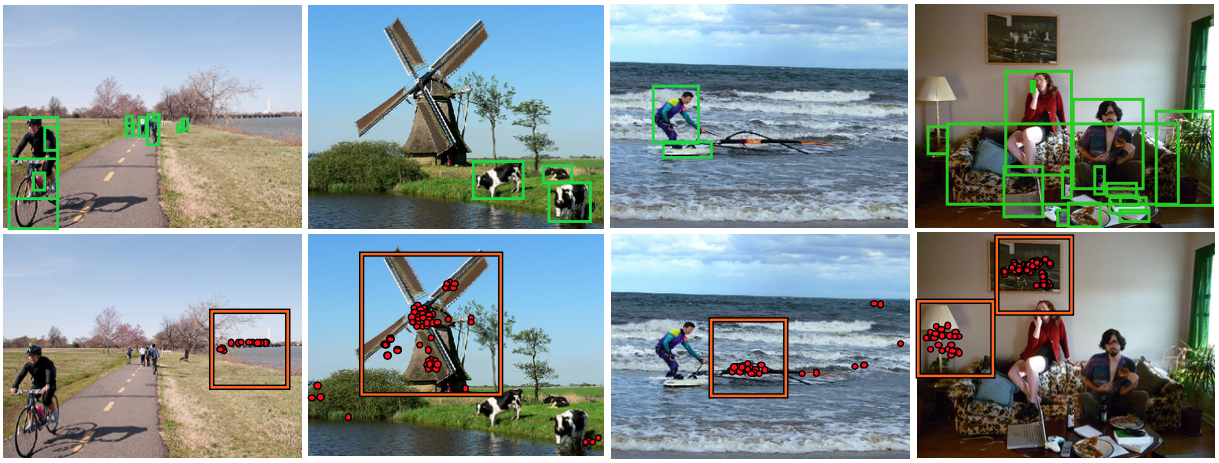
\includegraphics[width=13cm] {images/sniper_neg_chip}
        \caption{Kết quả thuật toán lựa chọn các negative chips (Nguồn: \cite{singh2018sniper})}
        \label{fig:sniper_pos_chip}
    \end{figure}

    \noindent
    Các bước lựa chọn negative Chips trong phương pháp SNIPER \index{SNIPER} như sau: \\
    \textit{Bước 1}: SNIPER \index{SNIPER} huấn luyện RPN của mô hình Faster R-CNN một vài epoch với chỉ các positive Chips. \\
    \textit{Bước 2}: SNIPER \index{SNIPER} sử dụng mô hình RPN đã được huấn luyện từ bước 1 để thực hiện dự đoán các khu vực đề xuất trong bộ dữ liệu huấn luyện (ảnh trong bộ dữ liệu huấn luyện lúc này cũng được thay đổi kích thước {${s}_{1}$, ..., ${s}_{n}$} như thuật toán lựa chọn positive Chips).
    Các khu vực không được RPN dự đoán sẽ được coi là những khu vực background \index{background} dễ học và loại các khu vực đó ra khỏi quá tình lựa chọn negative Chips. \\
    \textit{Bước 3}: Từ những khu vực mà RPN dự đoán, đầu tiên, SNIPER \index{SNIPER} loại các khu vực nằm trong danh sách positive Chips.
    Các Chips sẽ được lựa chọn nếu chứa nhiều hơn M khu vực được đề xuất tạo thành danh sách các negative Chips ${C}_{neg}^{i}$. \\
    \textit{Bước 4}: Danh sách các negative Chips được kết hợp cùng với danh sách các positive Chips để tiếp tục huấn luyện mô hình Faster R-CNN.

    \noindent
    \textbf{\textit{Kết quả của phương pháp chuẩn bị dữ liệu SNIPER \index{SNIPER}}} \\
    Theo thống kê của nhóm tác giả trên bộ dữ liệu COCO, bằng các phương pháp sinh và lựa chọn Chips, số lượng pixels \index{pixels} mà SNIPER \index{SNIPER} xử lý trong quá trình huấn luyện chỉ hơn khoảng 30\% so với số lượng pixels \index{pixels} cần xử lý khi huấn luyện với chỉ duy nhất một kích thước của ảnh.
    So sánh với việc huấn luyện với dữ liệu ảnh với 3 kích thước khác nhau cho mỗi ảnh, việc sử dụng các Chips có kích thước giống nhau giúp SNIPER \index{SNIPER} tối ưu về batch size hơn khi huấn luyện mô hình.
    So sánh với chiến lược của SNIP, SNIPER \index{SNIPER} đạt được độ chính xác tương đương trong khi giảm được 3 lần số pixels \index{pixels} cần phải huấn luyện trên bộ dữ liệu COCO.

    \noindent
    \textbf{\textit{Vấn đề tồn đọng của phương pháp chuẩn bị dữ liệu SNIPER \index{SNIPER}}} \\
    SNIPER \index{SNIPER} đã phần nào đó cải thiện một cách đáng kể vấn đề về thời gian huấn luyện của SNIP.
    Tuy nhiên, trong quá trình dự đoán, SNIPER \index{SNIPER} vẫn cần phải sử dụng phương pháp Image Pyramids để đạt được độ chính xác cao.
    Đối với những bộ dữ liệu ảnh có kích thước lớn thì tốc độ dự đoán của SNIPER \index{SNIPER} vẫn rất chậm và đây là vấn đề tồn đọng thúc đẩy các nghiên cứu giải quyết triệt để.
}
    \sniper

    \subsection{Mô hình AutoFocus}
    \def\autofocus{
    Từ vấn đề tồn đọng của phương pháp chuẩn bị dữ liệu SNIPER, mô hình AutoFocus \cite{najibi2019autofocus} đã ra đời nhằm tăng tốc quá trình dự đoán của mô hình object detection.
    AutoFocus hướng đến việc loại bỏ những pixel dư thừa mà mô hình phải xử lý trong quá trình dự đoán nhưng vẫn giữ được ý tưởng về việc sử dụng Image Pyramids.
    Mô hình AutoFocus được thiết kế nhằm dự đoán những khu vực đáng chú ý ở trên ảnh và loại bỏ những khu vực khả năng cao không chứa đối tượng ở những kích thước ảnh lớn hơn.
    Từ đó, tiết kiệm được rất nhiều chi phí tính toán trong quá trình predict của mô hình.

    \noindent
    \textbf{\textit{Kiến trúc tổng quá của mô hình AutoFocus}} \\
    Mô hình AutoFocus gồm hai nhánh: \\
    - Nhánh Focus (cụ thể gọi là Nhánh Focus Pixel Prediction) là nhánh mô hình giúp xác định được khu vực đáng chú ý trên ảnh để zoom to hơn, đồng thời loại bỏ các khu vực khả năng cao không chứa đối tượng. \\
    - Nhánh Detection là nhánh giúp mô hình định vị chính xác bounding box của từng đối tượng.
    Trong nghiên cứu, nhóm tác giả sử dụng mô hình Faster R-CNN \cite{ren2015faster} làm cơ sở cho nhánh Detection.

    \begin{figure}[H]
        \centering
        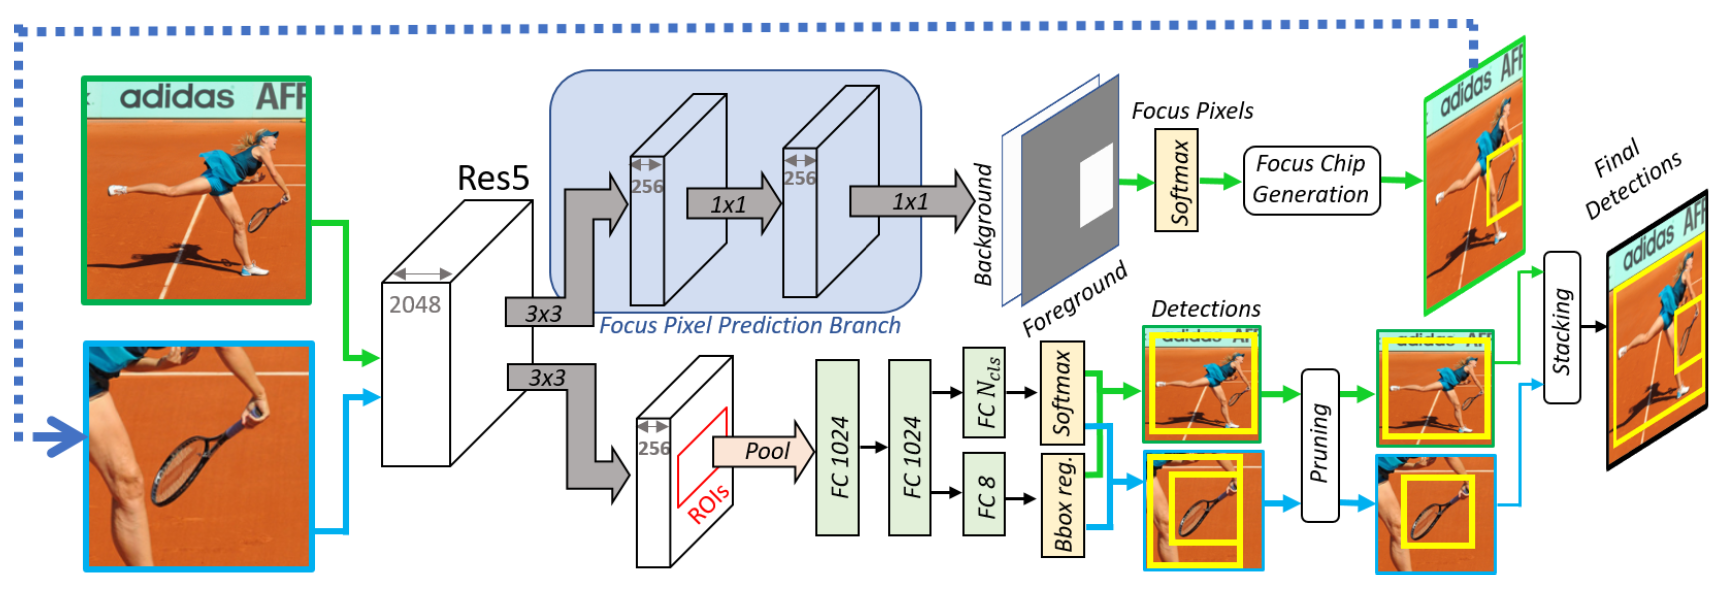
\includegraphics[width=15cm] {images/autofocus_model}
        \caption{Kiến trúc mô hình AutoFocus (Nguồn: \cite{najibi2019autofocus})}
        \label{fig:autofocus_model}
    \end{figure}
    
    \noindent
    Mô hình này nhận đầu vào xuất phát từ ảnh có kích thước nhỏ với mục tiêu định vị được những đối tượng có kích thước lớn và xác định khu vực khả năng cao chứa đối tượng.
    Với các khu vực khả năng cao chứa đối tượng, AutoFocus tiếp tục zoom vào với kích thước lớn hơn nhằm định vị được những đối tượng có kích thước nhỏ hơn và tiếp tục xác định khu vực khả năng cao chứa đối tượng.
    Quá trình này sẽ lặp đi lặp lại cho đến khi không còn khu vực nào cần phải zoom thì thuật toán sẽ dừng lại. \\
    Mô hình AutoFocus gồm ba thành phần là \textit{Thuật toán Focus Pixel} và \textit{Thuật toán sinh Focus Chips} thuộc nhánh Focus và \textit{Thuật toán Focus Stacking} thuộc nhánh Detection.

    \noindent
    \textbf{\textit{Thuật toán Focus Pixel}} \\
    Thuật toán Focus Pixel là thuật toán giúp chúng ta có thể xác định được vị trí khu vực có khả năng chứa đối tượng và cần zoom trên ảnh.
    Ý tưởng của thuật toán Focus Pixel dựa trên việc khi ta đưa đầu vào một ảnh có kích thước $X \times Y$ qua một khối Conv (như trong mô hình ResNet), feature maps mà ta thu được có kích thước $X' \times Y'$, trong đó: $X' = \lceil \frac{X}{s} \rceil$, $Y' = \lceil \frac{Y}{s} \rceil$, và $s$ là stride của cả khối Conv.
    Từ đó ta có thể ngầm hiểu rằng một pixel trên feature maps có kích thước $X' \times Y'$ đại diện cho một khu vực có kích thước $s \times s$ trên ảnh đầu vào. \\
    Với ý tưởng trên, từ groundtruth bounding box của đối tượng trên ảnh đầu vào, thuật toán Focus Pixel giúp xây dựng được label dạng mask của nhánh Focus với kích thước chiều dài chiều rộng bằng với khối Conv5 của mô hình backbone ResNet. \\
    Cụ thể hơn, Focus Pixel xác định các pixel trên mask là các \textit{pixel cần được focus} nếu như pixel đó có overlap với grountruth bounding box của đối tượng có kích thước nhỏ.
    Tiếp theo, các pixel trên mask là các \textit{pixel không cần quan tâm} nếu như pixel đó có overlap với groundtruth bounding box của đối tượng có kích thước lớn hoặc rất nhỏ.
    Cuối cùng, các \textit{pixel không cần được focus} trên mask là các pixel còn lại.

    \[l = 
        \begin{cases}
            1, & IoU(GT, l) > 0, a < \sqrt{GTArea} < b \\
            -1, & IoU(GT, l) > 0, \sqrt{GTArea} < a  \\
            -1, & IoU(GT, l) > 0, b < \sqrt{GTArea} < c  \\
            0, & \text{otherwise}
        \end{cases}
    \]

    \noindent
    trong đó: \\
    - $IoU(GT, l)$ là chỉ số IoU giữa khu vực $s \times s$ và groundtruth bounding box của đối tượng trên ảnh đầu vào. \\
    - $GTArea$ là diện tích của groundtruth bounding box của đối tượng trên ảnh đầu vào. \\
    Nếu một khu vực $s \times s$ overlap với nhiều groundtruth bounding box của đối tượng, thì pixel đó được ưu tiên là một Focus Pixel.

    \begin{figure}[H]
        \centering
        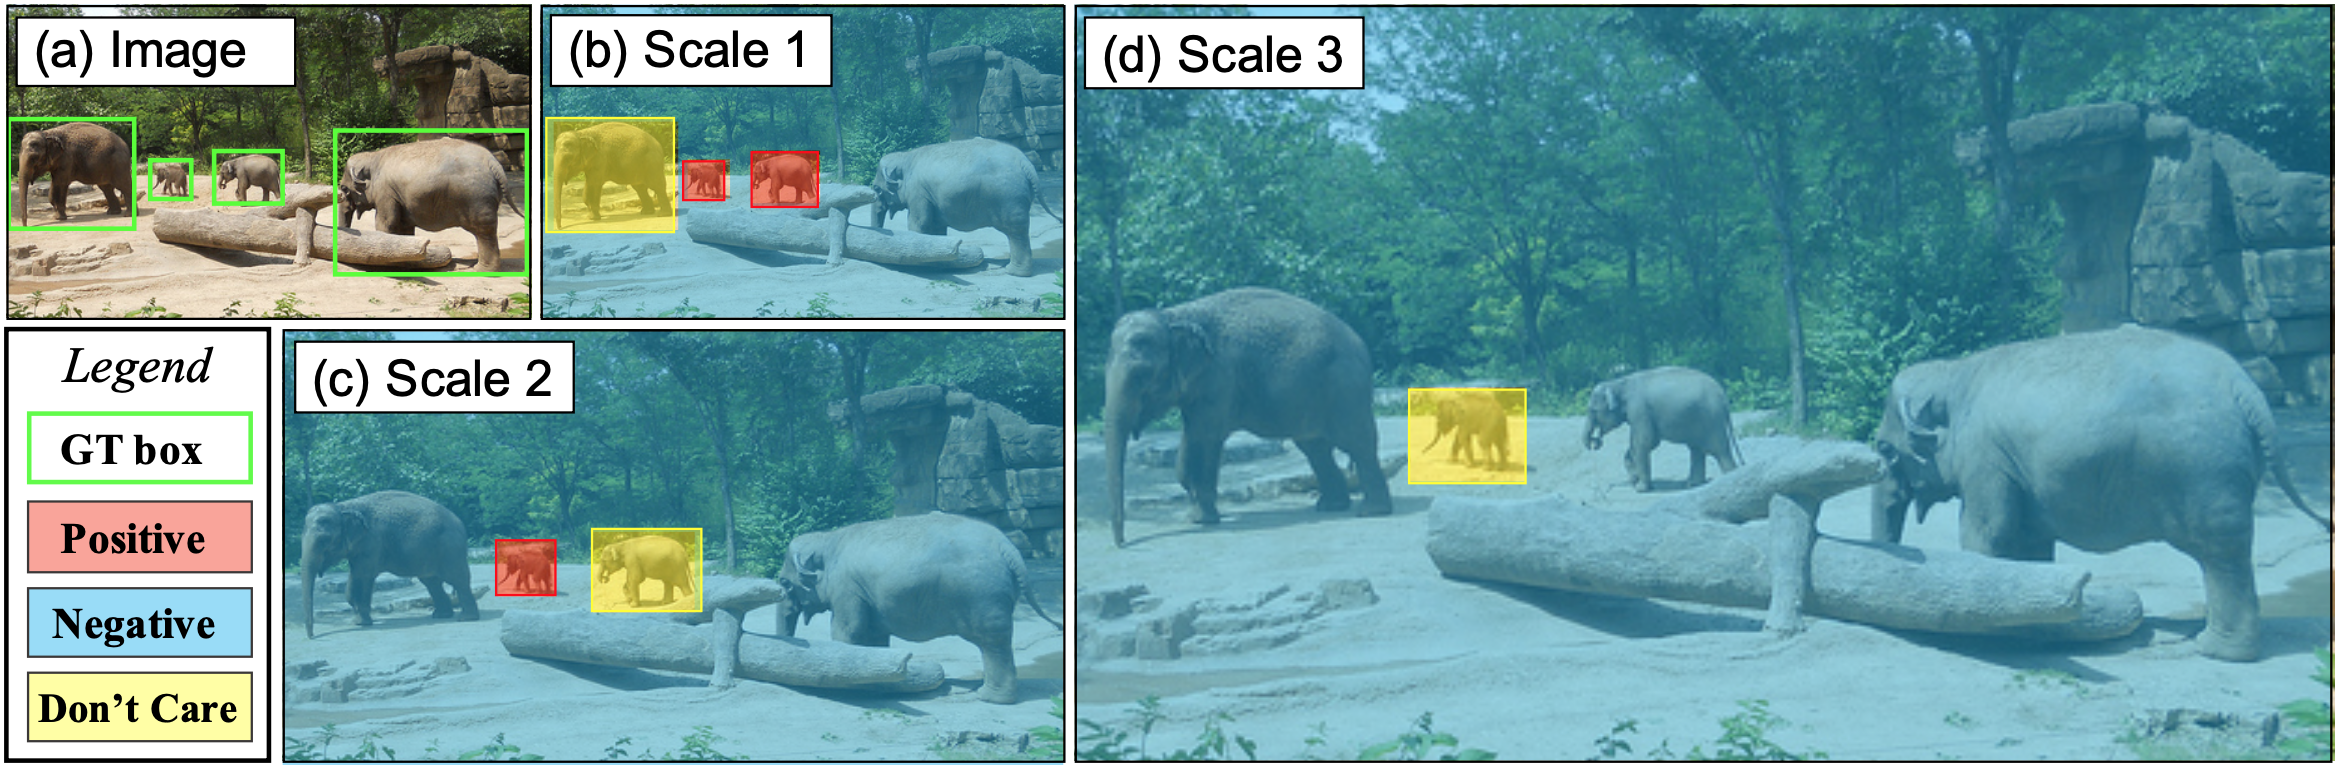
\includegraphics[width=15cm] {images/autofocus_focus_pixel}
        \caption{Ví dụ về cơ chế hoạt động của thuật toán Focus Pixel (Nguồn: \cite{najibi2019autofocus})}
        \label{fig:autofocus_focus_pixel}
    \end{figure}

    \noindent
    Trong các thí nghiệm mà nhóm tác giả thực hiện trong nghiên cứu, nhóm tác giả sử dụng ảnh đầu vào có kích thước $512 \times 512$, với các tham số $a = 5, b = 64, c = 90$ nghĩa là các groundtruth bounding box có kích thước từ $5 \times 5$ đến $64 \times 64$ là các bounding box cần được focus, các groundtruth bounding box có kích thước dưới $5 \times 5$ hoặc từ $64 \times 64$ đến $90 \times 90$ là các bounding box không cần quan tâm và các groundtruth bounding box có kích thước trên $90 \times 90$ là các bounding box không cần được focus.
    Từ các tham số trên, tỷ lệ giữa các \textit{pixel cần được focus} và \textit{pixel không cần được focus} là 10.

    \noindent
    \textbf{\textit{Thuật toán sinh Focus Chips}} \\
    Sau khi mô hình đã được train và predict ra được pixel cần được focus, mô hình cần một thuật toán để crop ra được khu vực cần focus trên ảnh làm đầu vào cho mô hình AutoFocus lượt tiếp theo.
    Và đó là vai trò của thuật toán sinh Focus Chips.

    \begin{figure}[H]
        \centering
        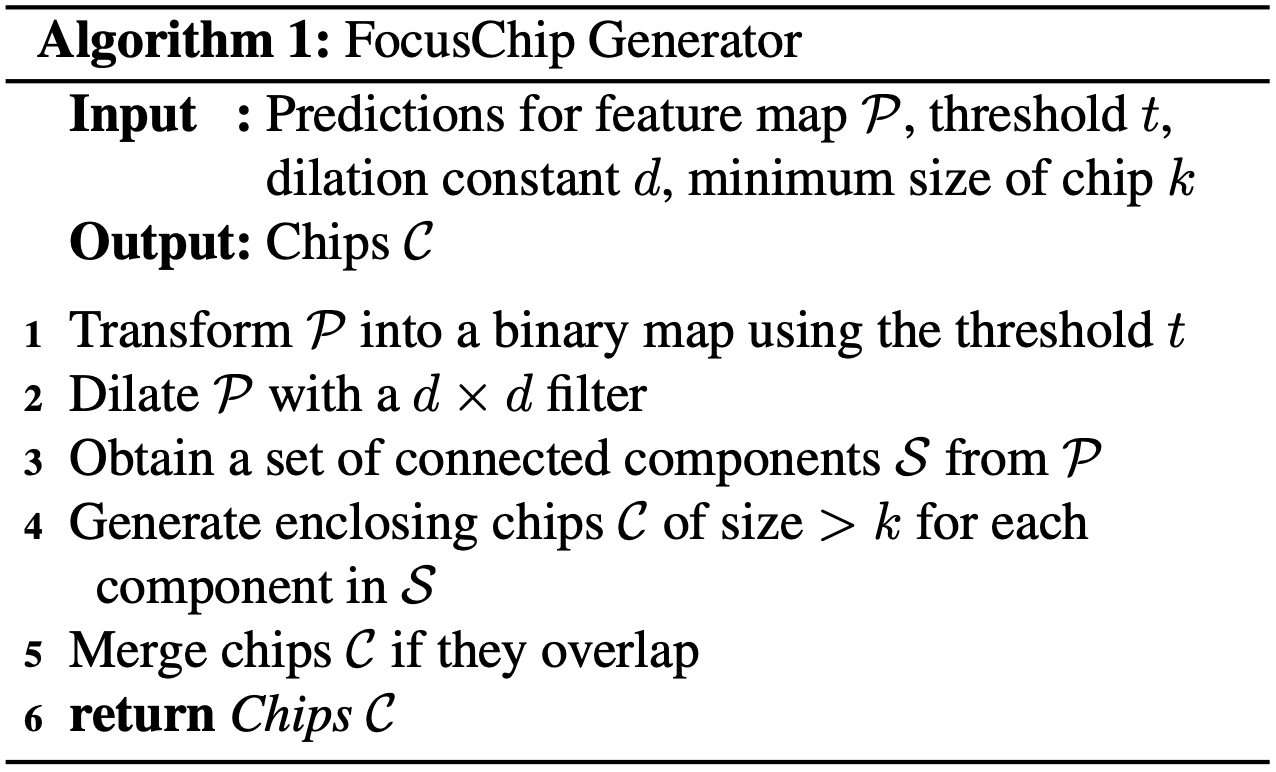
\includegraphics[width=10cm] {images/autofocus_focus_chip_gen}
        \caption{Chi tiết thuật toán sinh Focus Chips (Nguồn: \cite{najibi2019autofocus})}
        \label{fig:autofocus_focus_chip_gen}
    \end{figure}

    \noindent
    Trong quá trình predict, sau khi mô hình đã predict được các pixel cần được focus (ký hiệu là $\mathcal{P}$) trên Focus Pixel mask, ta biến đổi mask này trở về dạng binary mask bằng threshold $t$.
    Tham số $t$ được sử dụng để cân đối giữa tốc độ và độ chính xác của mô hình (cụ thể với tham số $t$ lớn, số lượng các pixel cần được focus sẽ giảm đi và tốc độ của mô hình AutoFocus sẽ tăng và ngược lại). \\
    Từ binary mask đã được sinh ra ở trên, thuật toán sinh Focus Chips sẽ đưa qua một filter có kích thước $d \times d$ nhằm giãn nở các pixel thêm một chút để thu được các thành phần liên thông $\mathcal{S}$, từ đó có nhiều thông tin hơn khi crop ảnh đầu vào với các focus pixel này. \\
    Cuối cùng, ta crop ra các chip $\mathcal{C}$ với kích thước tối thiểu là $k \times k$ và bao trọn các thành phần liên thông $\mathcal{S}$ trên.
    Các chip trong $\mathcal{C}$ nếu có overlap với nhau sẽ được gộp lại chung thành một chip. \\
    Việc sinh ra các chip $\mathcal{C}$ giúp mô hình AutoFocus có thể sử dụng ý tưởng Image Pyramids nhưng tiết kiệm chi phí tính toán nhờ loại bỏ các khu vực khả năng cao không chứa đối tượng.

    \noindent
    \textbf{\textit{Thuật toán Focus Stacking}} \\
    Một vấn đề cần phải giải quyết khi thực hiện predict với ý tưởng Image Pyramids trong bài toán object detection là việc tổng hợp lại các bounding box.
    Đối với mô hình AutoFocus, vấn đề này còn phức tạp hơn với trường hợp một đối tượng có kích thước lớn được dự đoán ở kích thước này, nhưng đến kích thước tiếp theo, đối tượng đó bị crop trong quá trình crop chip và trở thành một đối tượng có kích thước nhỏ hơn.
    Nhằm hạn chế bớt vấn đề này, nhóm tác giả chỉ ra rằng \textit{bước 2} trong thuật toán sinh Focus Chips \ref{fig:autofocus_focus_chip_gen} là cực kỳ quan trọng.

    \begin{figure}[H]
        \centering
        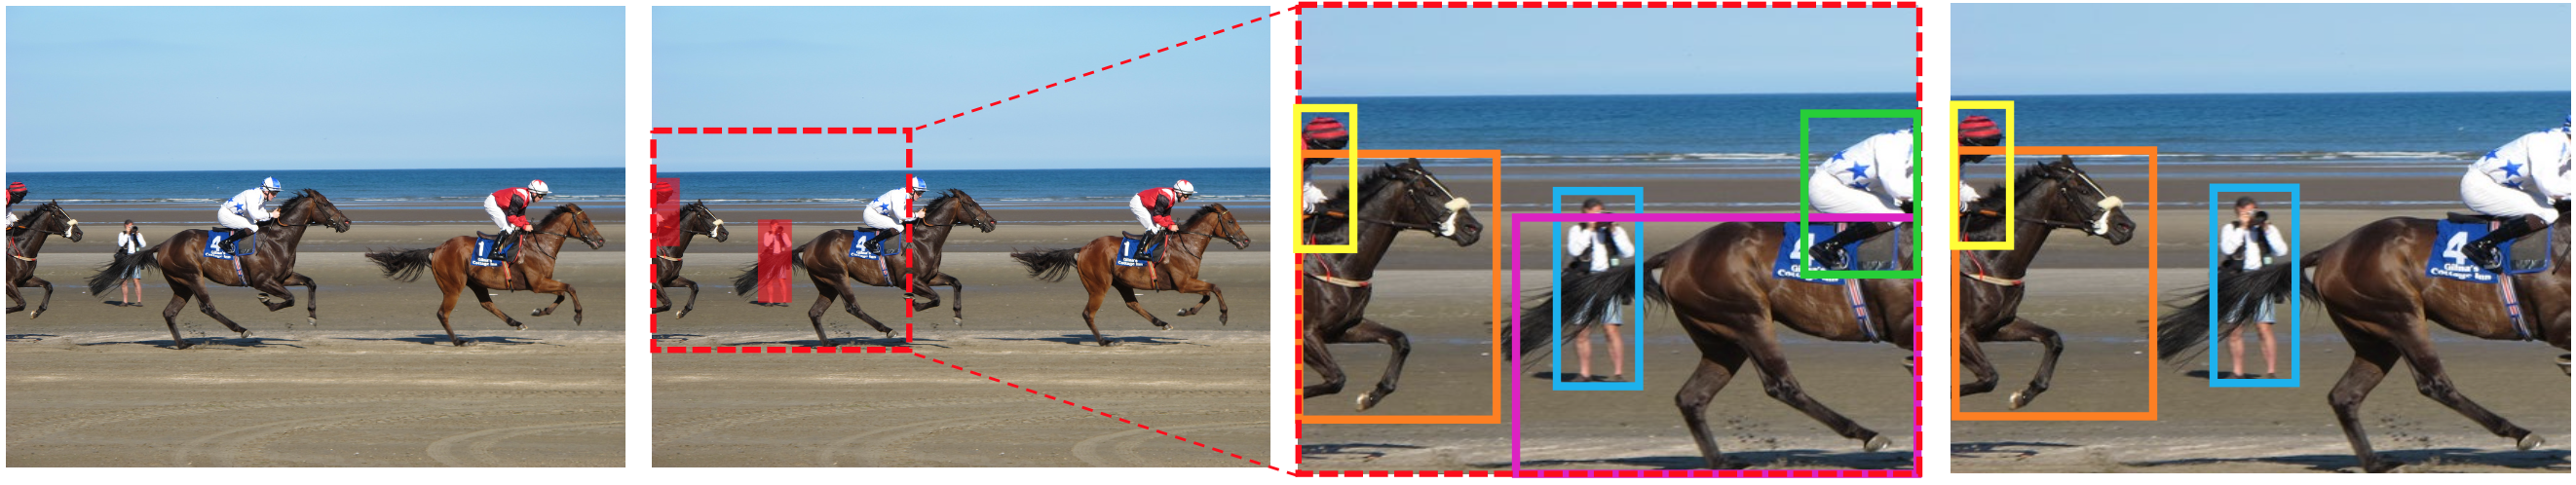
\includegraphics[width=10cm] {images/autofocus_focus_stack}
        \caption{Ví dụ về cơ chế hoạt động của thuật toán Focus Stacking (Nguồn: \cite{najibi2019autofocus})}
        \label{fig:autofocus_focus_stack}
    \end{figure}

    \noindent
    Tuy nhiên, nhóm tác giả cũng đề ra một số luật nhằm loại bỏ các dự đoán lỗi của các đối tượng được định vị trên một focus chip: \\
    - Nếu một đối tượng nằm trên một biên của chip nhưng không phải biên của ảnh đầu vào (nghĩa là đối tượng này đã bị crop sau khi qua thuật toán sinh Focus Chip), thì dự đoán sẽ bị loại bỏ. \\
    - Nếu một đối tượng nằm trên một biên của chip và đó là biên của ảnh đầu vào, nhóm tác giả sẽ tiếp tục kiểm tra biên còn lại của đối tượng, nếu đó là biên của chip, dự đoán sẽ bị loại, còn nếu đó không phải là biên của chip, dự đoán sẽ được giữ lại. \\
    - Nếu một đối tượng nằm trên hai biên của chip và đó đều là hai biên của ảnh đầu vào, nhóm tác giả sẽ giữ lại những dự đoán này. \\
    Sau khi loại bỏ bớt các dự đoán bằng thuật toán Focus Stacking, mô hình AutoFocus đưa ra tổng hợp dự đoán từ các kích thước ảnh khác nhau và là các dự đoán cuối cùng của ảnh đầu vào.

    \noindent
    \textbf{\textit{Kết quả của mô hình AutoFocus}} \\
    Kết quả của mô hình AutoFocus so sánh với các mô hình khác là rất ấn tượng trên bộ dữ liệu COCO test-dev.
    Số lượng pixel mà mô hình cần xử lý được chú thích tại cột \textit{Pixels}.
    Mô hình AutoFocus giữ được kết quả tương đương với mô hình sử dụng phương pháp chuẩn bị dữ liệu SNIPER trên tất cả các chỉ số trong khi đạt số lượng pixel cần xử lý ít hơn nhiều so với mô hình sử dụng SNIPER.

    \begin{figure}[H]
        \centering
        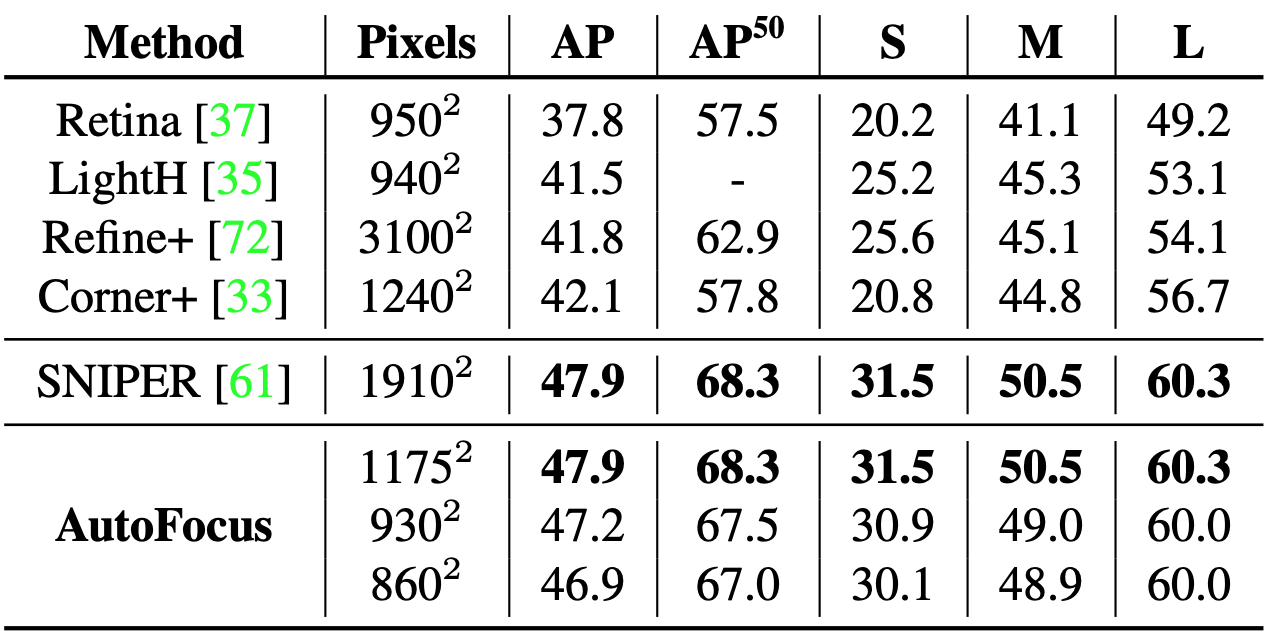
\includegraphics[width=10cm] {images/autofocus_results_1}
        \caption{Kết quả của mô hình AutoFocus so sánh với các mô hình khác trên bộ dữ liệu COCO test-dev (Nguồn: \cite{najibi2019autofocus})}
        \label{fig:autofocus_results_1}
    \end{figure}

    \noindent
    Nhóm tác giả chia sẻ rằng dù đạt kết quả là 47.9\% tương đương với SNIPER, nhưng AutoFocus có khả năng xử lý khoảng 6.4 ảnh/giây trên bộ COCO test-dev trên Titan X Pascal GPU so sánh với chỉ 2.5 ảnh/giây của mô hình sử dụng SNIPER. \\
    Mô hình RetinaNet với ResNet-101 backbone đạt tốc độ gần tương đương với AutoFocus là 6.4 ảnh/giây trên bộ COCO test-dev trên P100 GPU (tương đương với Titan X Pascal GPU) nhưng chỉ đạt mức mAP là 37.8\%.
    Nhóm tác giả cũng nhấn mạnh rằng AutoFocus là mô hình nhanh nhất ở thời điểm đó xử lý bộ dữ liệu COCO và đạt chỉ số mAP là 47.9\%.

    \begin{figure}[H]
        \centering
        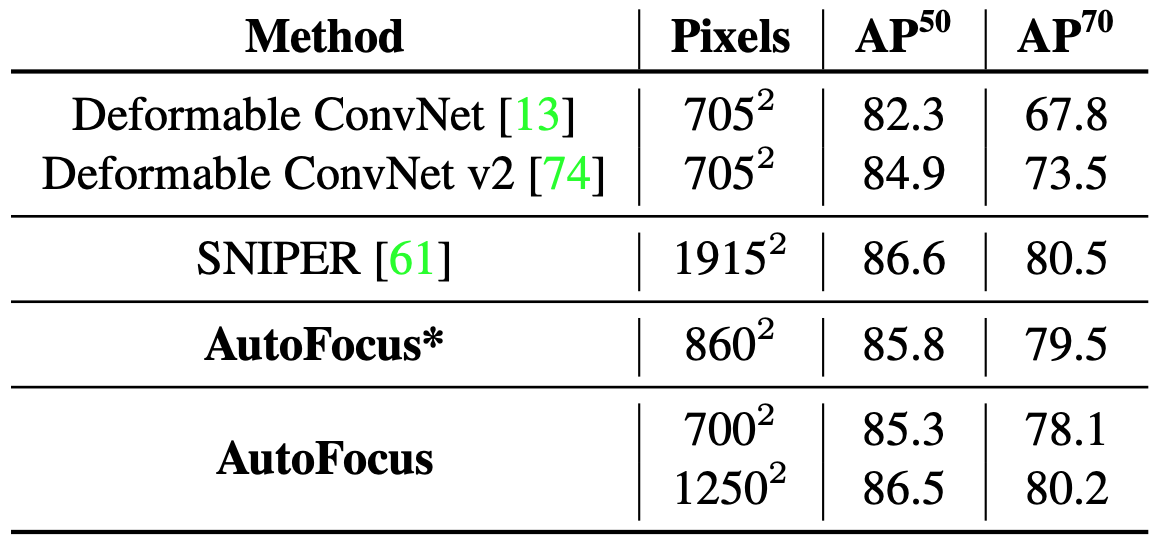
\includegraphics[width=10cm] {images/autofocus_results_2}
        \caption{Kết quả của mô hình AutoFocus so sánh với các mô hình khác trên bộ dữ liệu PASCAL VOC 2007 test-set (Nguồn: \cite{najibi2019autofocus})}
        \label{fig:autofocus_results_2}
    \end{figure}

    \noindent
    Kết quả của mô hình AutoFocus so sánh với các mô hình khác trên bộ dữ liệu PASCAL VOC 2007 test-set cũng được nhóm tác giả chia sẻ.
    Ở đây, nhóm tác giả cũng nhấn mạnh vào sức mạnh của mô hình AutoFocus khi sử dụng cấu hình được finetune của mô hình trên bộ dữ liệu COCO (mô hình ký hiệu là AutoFocus*) để giải quyết bộ dữ liệu PASCAL VOC 2007 nhưng vẫn đạt kết quả tốt.

    \begin{figure}[H]
        \centering
        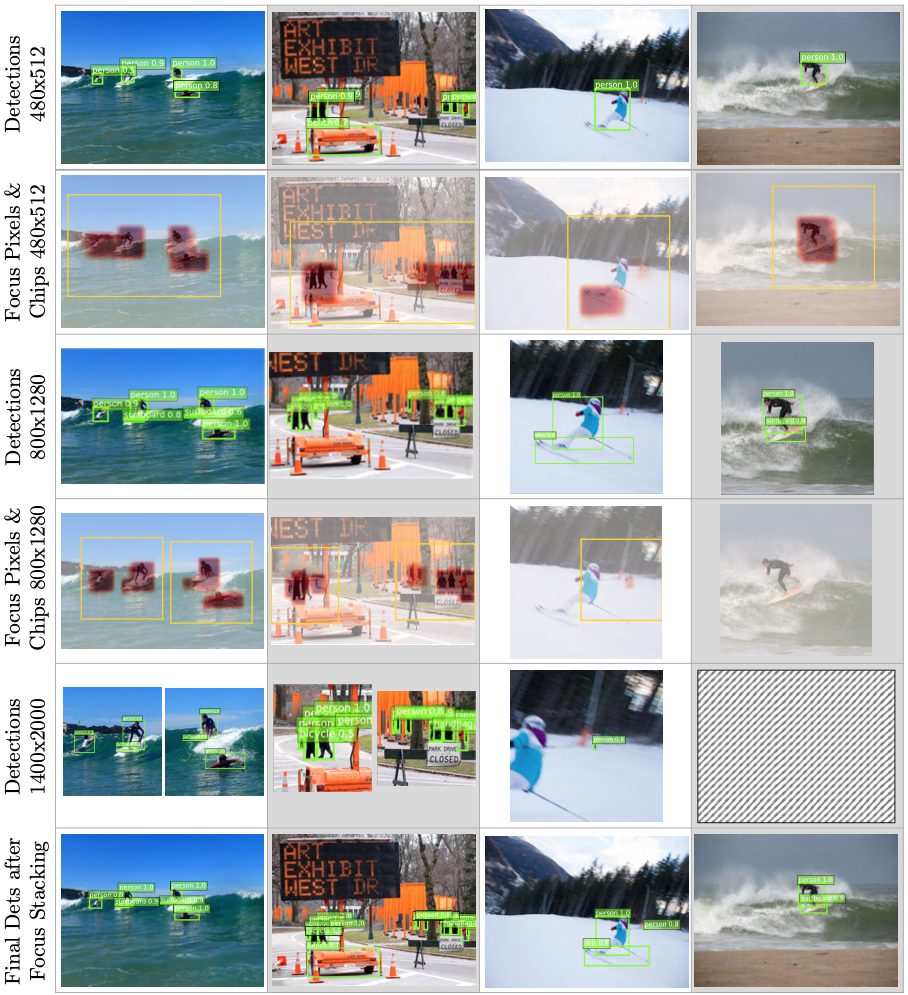
\includegraphics[width=10cm] {images/autofocus_results_3}
        \caption{Từng bước quá trình dự đoán của mô hình AutoFocus với một số ảnh trong bộ dữ liệu COCO val-2017(Nguồn: \cite{najibi2019autofocus})}
        \label{fig:autofocus_results_3}
    \end{figure}

    \noindent
    \textbf{\textit{Vấn đề tồn đọng của mô hình AutoFocus}} \\
    Nghiên cứu của mô hình AutoFocus đã mang lại một ý tưởng rất thông minh để xử lý rất nhanh bài toán object detection với ảnh chất lượng cao trong khi vẫn duy trì được độ chính xác cao, tương đương với các mô hình sử dụng phương pháp Image Pyramids truyền thống.
    Tuy nhiên, mô hình AutoFocus vẫn tồn tại điểm yếu khá lớn là số lượng hyperpameter của mô hình nhiều.
    Điều này gây ra khó khăn trong việc tìm kiếm một cấu hình tốt nhất của mô hình đối với từng bài toán hay từng bộ dữ liệu khác nhau.
    Nghiên cứu và phân tích về điểm yếu này sẽ được trình bày trong phần sau của luận văn.
}
    \autofocus
}
    \objectdetectionhighres

    \newpage
    \def\facedetectionhighres{
    \section{Các mô hình giải quyết bài toán Face Detection trong ảnh chất lượng cao}

    \subsection{Mô hình RetinaFace}
    RetinaFace \cite{deng2020retinaface} là một mô hình single-stage giải quyết bài toán Face Detection.
    RetinaFace có kiến trúc mô hình \ref{fig:retinaface_architecture} khá giống với RetinaNet (đã được nêu trong phần)
    TODO: ref phần RetinaNet

    \begin{figure}[H]
        \centering
        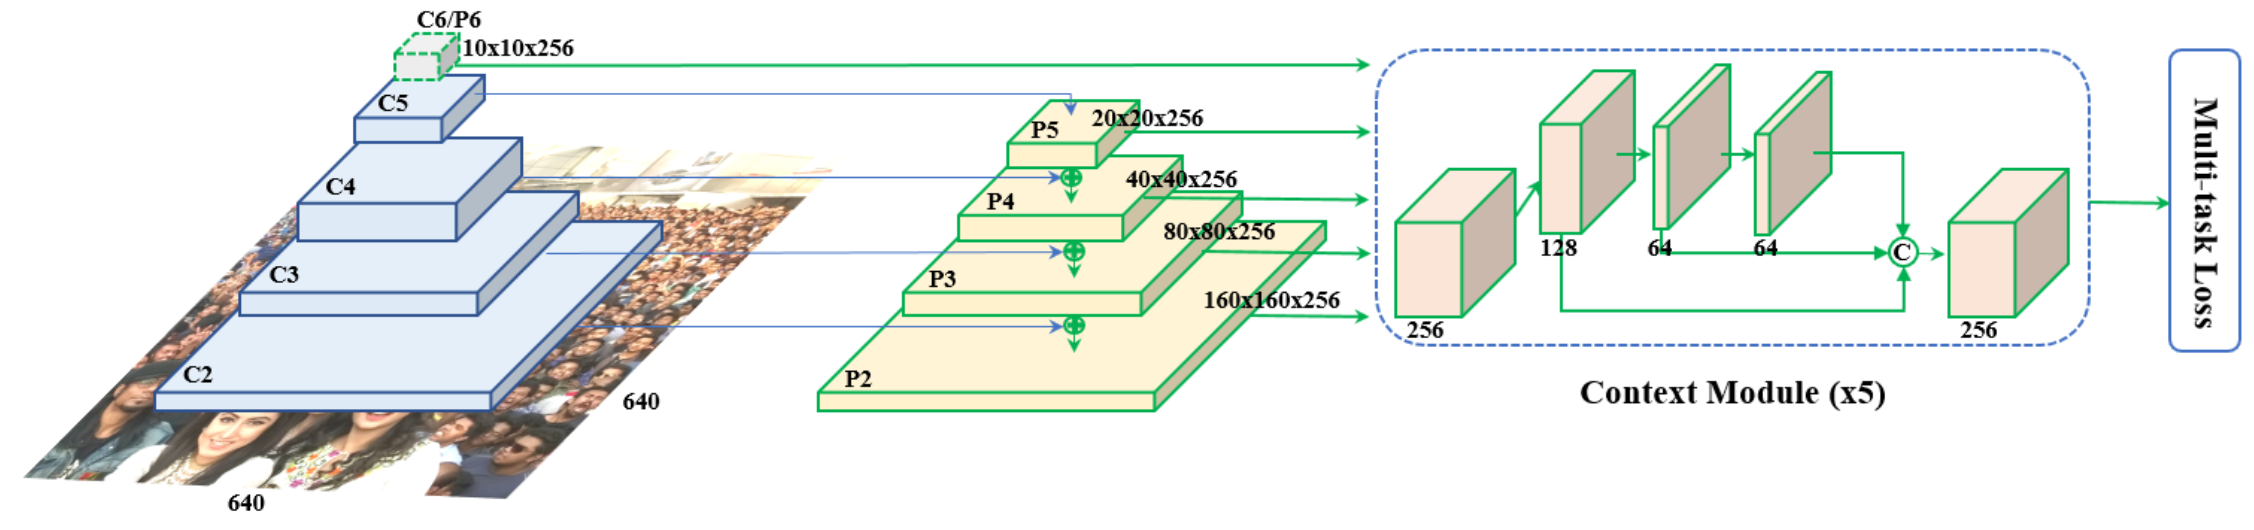
\includegraphics[width=10cm] {images/retinaface_architecture.png}
        \caption{Kiến trúc của mô hình RetinaFace}
        \label{fig:retinaface_architecture}
    \end{figure}

    Nhóm tác giả của RetinaFace đã mang đến bộ dữ liệu và một số kỹ thuật mới giúp cải thiện hiệu năng giải quyết bài toán Face Detection như bộ dữ liệu WIDER FACE với landmarks, 
    TODO: Bổ sung tên các techniques của RetinaFace
    \subsubsection{Bộ dữ liệu WIDER FACE với landmarks}
    \textbf{\textit{Bộ dữ liệu WIDER FACE nguyên bản}} \\
    Bộ dữ liệu WIDER FACE \cite{yang2016wider} là một bộ dữ liệu nổi tiếng dành cho bài toán Face Detection.
    Bộ dữ liệu này bao gồm 32,203 ảnh được chụp từ 61 khung cảnh khác nhau với 393,703 bbox của khuôn mặt với sự đa dạng trong tỷ lệ kích thước, kiểu dáng, biểu cảm, che chắn và ánh sáng.
    WIDER FACE được chia ngẫu nhiêu thành 3 phần, trong đó: phần dữ liệu train chiếm 40\%, phần dữ liệu val chiếm 10\% và phần dữ liệu test chiếm 50\%. \\
    Nhóm tác giả của bộ dữ liệu WIDER FACE sử dụng mô hình EdgeBox \cite{zitnick2014edge} để chia bộ dữ liệu thành ba mức độ khó (bộ Dễ, bộ Trung bình và bộ Khó). \\
    TODO: Nói thêm về cách chia thành 3 mức khó, Nói thêm về mô hình EdgeBox \\
    \textbf{\textit{Bộ dữ liệu WIDER FACE với landmarks}} \\
    Nhóm tác giả của RetinaFace đã bổ sung thêm vào bộ dữ liệu WIDER FACE thông tin về landmarks của các khuôn mặt bao gồm 5 điểm: tâm của mắt trái, tâm của mắt phải, đỉnh của mũi, điểm mép miệng trái và điểm mép miệng phải.
    Dựa vào chất lượng của ảnh (cụ thể là mức độ khó để có thể nhận ra được 5 điểm landmarks nói trên), nhóm tác giả đã chia bộ dữ liệu thành 5 mức độ khó, chi tiết được biểu diễn thông qua Hình \ref{fig:retinaface_widerface} và Bảng.
    Nhóm tác giả của RetinaFace đã gán landmarks cho các khuôn mặt trong hai tập dữ liệu train và val (tương ứng 84.6k mặt cho tập train và 18.5k mặt cho bộ val).
    
    \begin{figure}[H]
        \centering
        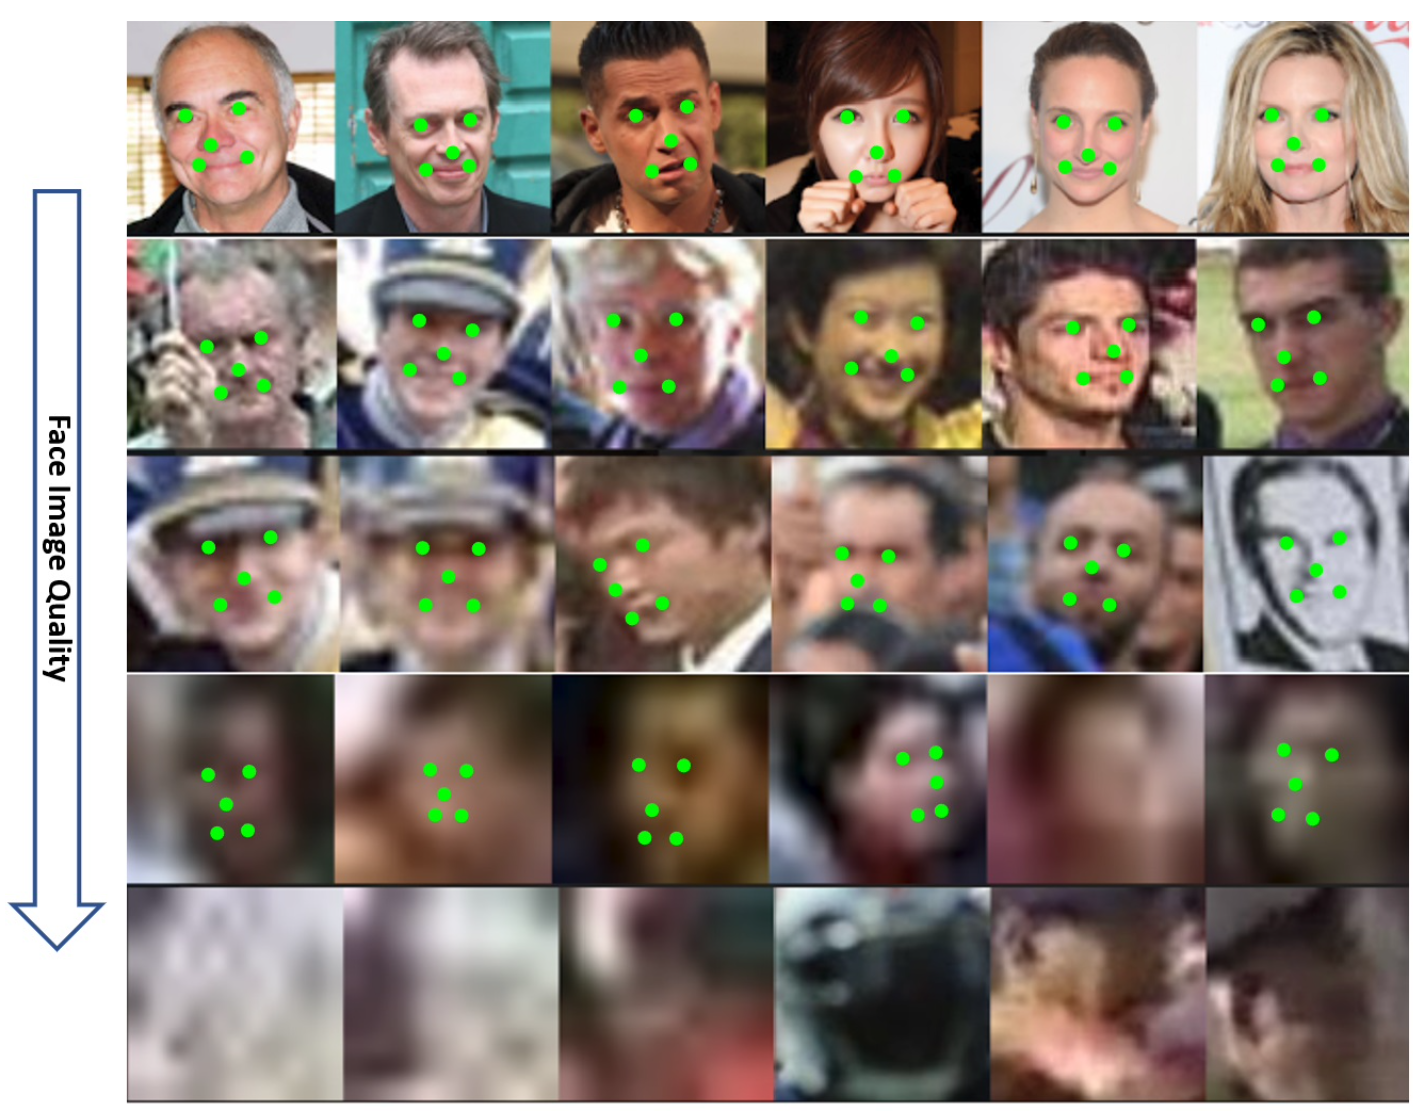
\includegraphics[width=10cm] {images/retinaface_widerface.png}
        \caption{Ví dụ về năm mức độ khó của khuôn mặt trong việc gán landmarks theo RetinaFace}
        \label{fig:retinaface_widerface}
    \end{figure}

    \begin{table}[ht!]
        \centering
        \begin{tabular}{l|c|c}
            \hline
            Level            & Face Number &  Criterion\\
            \hline
            1 & 4,127  & indisputable 68 landmarks~\cite{sagonas2013300} \\
            2 & 12,636 & annotatable 68 landmarks~\cite{sagonas2013300} \\
            3 & 38,140 & indisputable 5 landmarks\\
            4 & 50,024 & annotatable 5 landmarks\\
            5 & 94,095 & distinguish by context  \\
            \hline
        \end{tabular}
        \hspace{1in}
        \caption{Five levels of face image quality. In the indisputable category a human can, without a lot of effort, locale the landmarks. In the annotatable category  finding an approximate location requires some effort.}
        \label{tab:fivelevel}
        \vspace{-4mm}
    \end{table}


    \subsubsection{Hàm loss multi-task}
    Trong quá trình train mô hình, với mỗi anchor, RetinaFace tối ưu hàm loss multi-task dưới đây:
    \begin{equation}
        \begin{split}
        L  & =  L_{cls}(p_i, p^{*}_i) + \lambda_1 p^{*}_i L_{box}(t_i, t^{*}_i) + \lambda_2 p^{*}_i L_{pts} (l_i, l^{*}_i) + \lambda_3 p^{*}_i L_{pixel}.\\
        \end{split}
        \label{eq:loss}
    \end{equation}
    Hàm loss trên được gọi là multi-task loss bởi vì nó cùng lúc tối ưu mô hình RetinaFace theo nhiều bài toán con.
    Ta có bốn số hạng của hàm loss tổng, tương ứng với đó là bốn bài toán con mà mô hình sẽ tối ưu: \\
    Phần 1 là hàm loss phân lớp mặt (cụ thể hơn là hàm loss softmax phân lớp nhị phân \textit{là mặt / không là mặt}):
    $L_{cls}(p_i, p^{*}_i)$ với $p_i$ là xác suất mà mô hình dự đoán một anchor có phải là mặt hay không.
    Ta có $p^{*}_i = 1$ nếu anchor đó là mặt còn $p^{*}_i = 0$ nếu anchor đó không phải là mặt. \\
    Phần 2 là hàm loss hồi quy định vị vị trí của bbox:
    $L_{box}(t_i, t^{*}_i)$ với $t_i=\{t_x, t_y, t_w, t_h\}_i$ và $t^{*}_i=\{t^{*}_x, t^{*}_y, t^{*}_w, t^{*}_h\}_i$ lần lượt là bộ bốn tham số đại diện cho toạ độ của anchor mà mô hình dự đoán là mặt và bbox ground-truth từ bộ dữ liệu.
    (toạ độ x của điểm góc trái trên, toạ độ y của điểm góc trái trên, chiều rộng của bbox và chiều cao của bbox)
    We follow~\cite{girshick2015fast} to normalise the box regression targets (centre location, width and height) and use $L_{box}(t_i, t^{*}_i)=R(t_i - t^{*}_i)$, where $R$ is the robust loss function (smooth-L$_1$) defined in~\cite{girshick2015fast}. 
    Phần 3 là hàm loss hồi quy định vị vị trí của landmarks:
    $L_{pts} (l_i, l^{*}_i)$ với $l_i=\{l_{x_1}, l_{y_1}, \dots , l_{x_5}, l_{y_5}\}_i$ và $l^{*}_i=\{l^{*}_{x_1}, l^{*}_{y_1}, \dots , l^{*}_{x_5}, l^{*}_{y_5}\}_i$ represent the predicted five facial landmarks and ground-truth associated with the positive anchor. 
    Similar to the box centre regression, the five facial landmark regression also employs the target normalisation based on the anchor centre.
    (4) Dense regression loss $L_{pixel}$ (refer to Eq.~\ref{fig:selfsupervision}).  
    The loss-balancing parameters $\lambda_1$-$\lambda_3$ are set to 0.25, 0.1 and 0.01, which means that we increase the significance of better box and landmark locations from supervision signals.

    \subsubsection{Kết quả của mô hình RetinaFace}
    \textbf{\textit{Đ}}

    \begin{figure*}[t]
        \centering
        \subfigure[Tập dữ liệu val Dễ]{
        \label{fig:ve}
        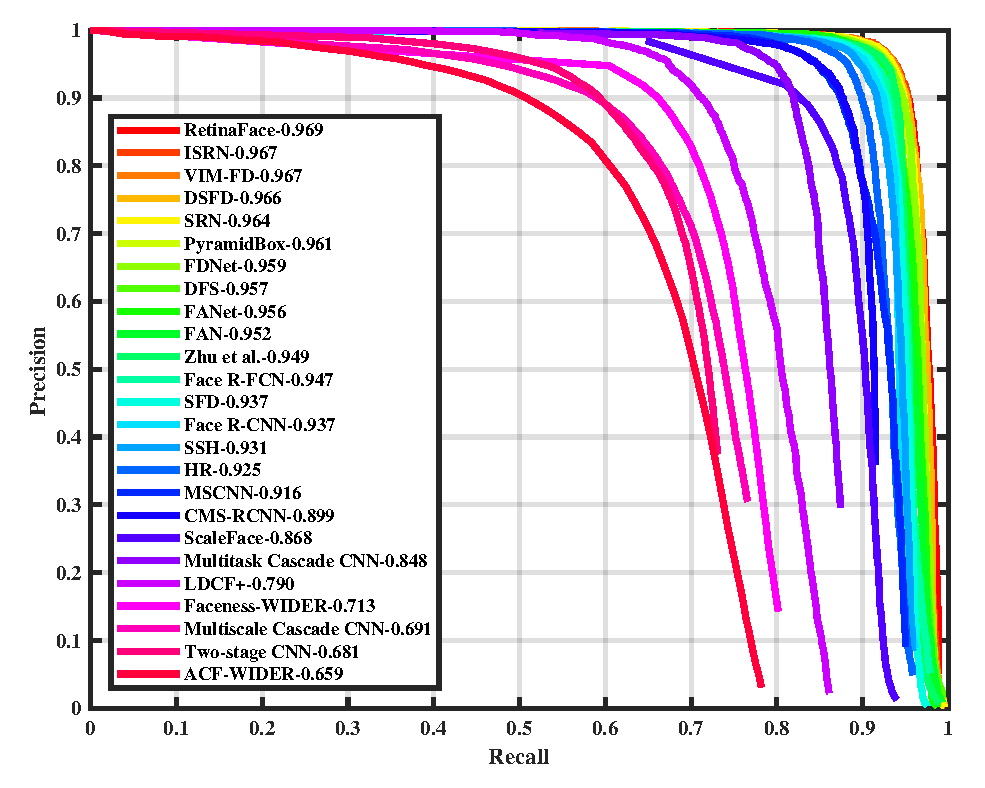
\includegraphics[width=0.32\linewidth]{images/vale.pdf}}
        \subfigure[Tập dữ liệu val Trung bình]{
        \label{fig:vm}
        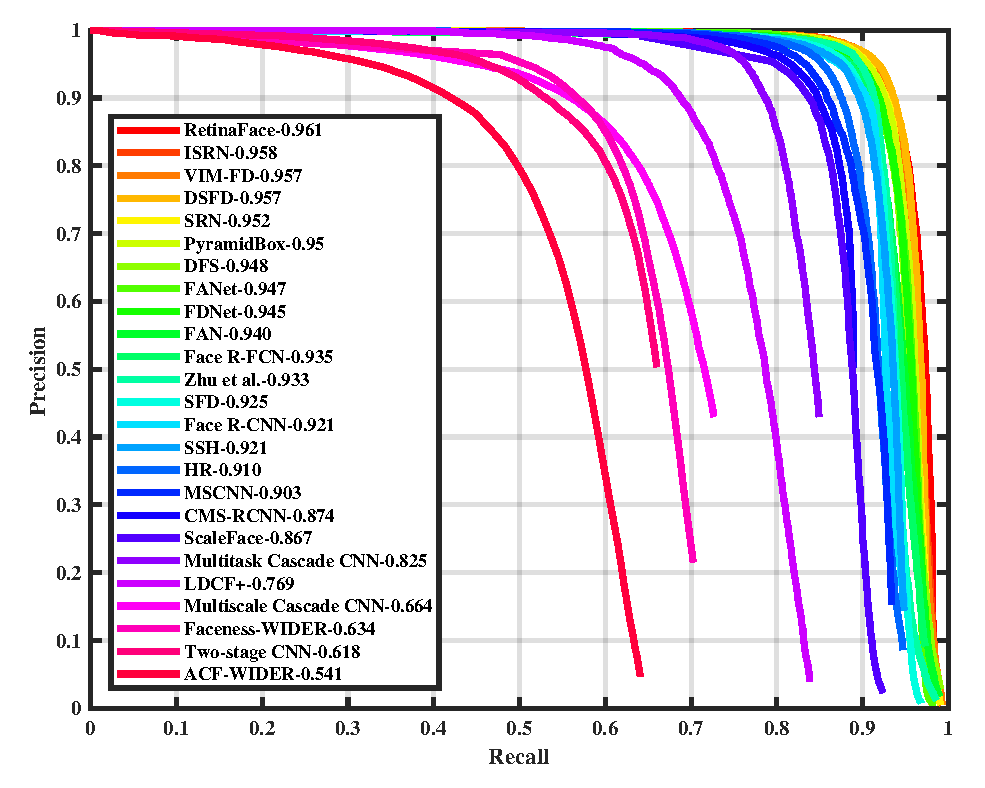
\includegraphics[width=0.32\linewidth]{images/valm.pdf}}
        \subfigure[Tập dữ liệu val Khó]{
        \label{fig:vh}
        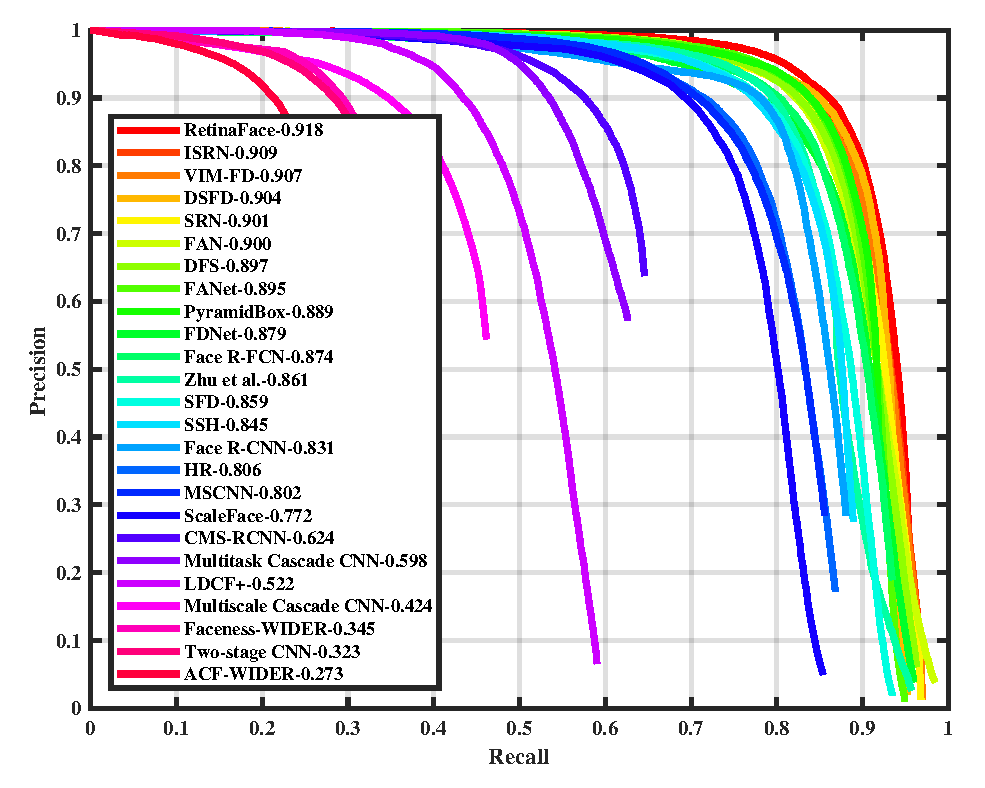
\includegraphics[width=0.32\linewidth]{images/valh.pdf}}
        \subfigure[Tập dữ liệu test Dễ]{
        \label{fig:te}
        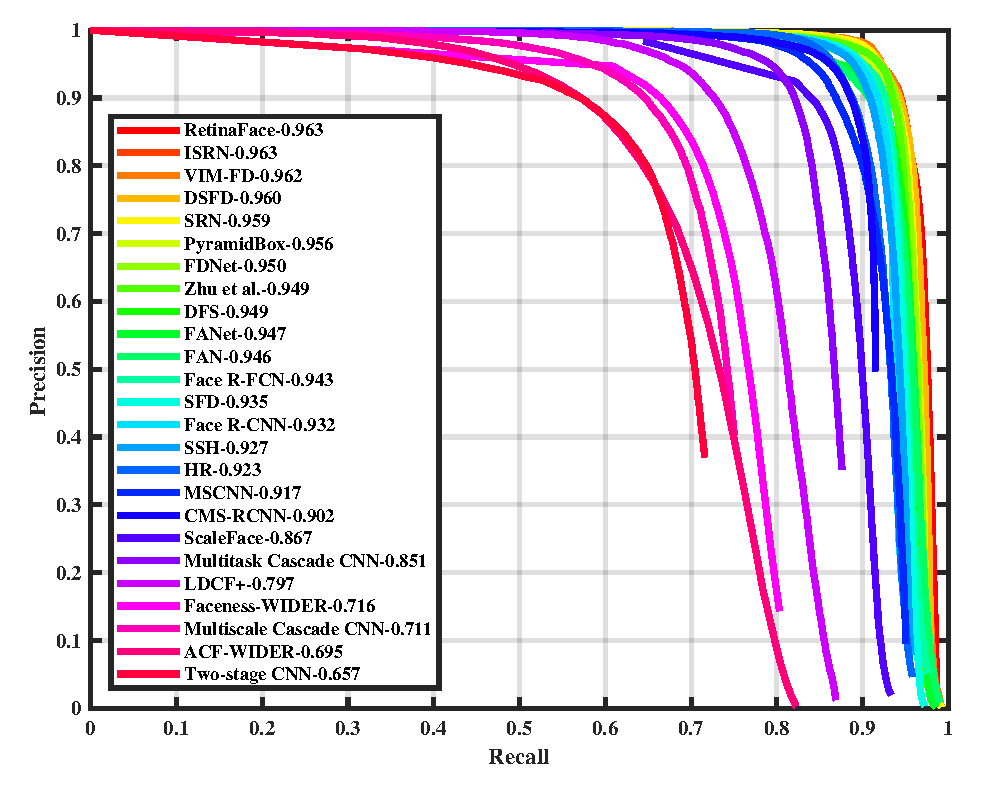
\includegraphics[width=0.32\linewidth]{images/te.pdf}}
        \subfigure[Tập dữ liệu test Trung bình]{
        \label{fig:tm}
        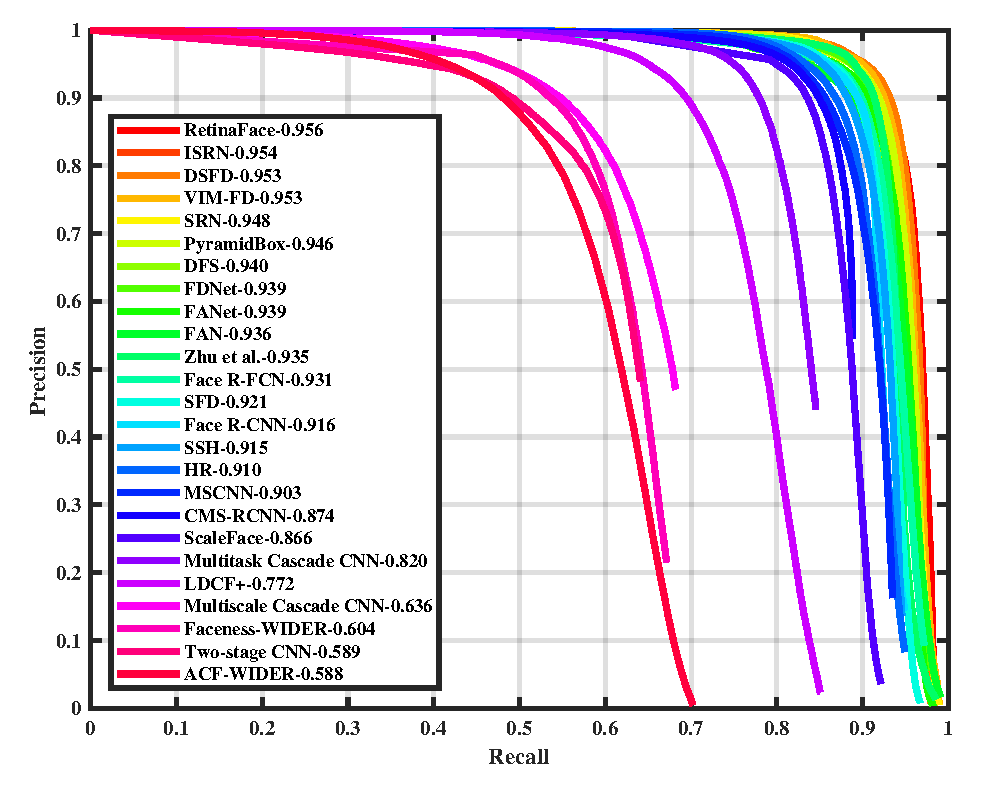
\includegraphics[width=0.32\linewidth]{images/tm.pdf}}
        \subfigure[Tập dữ liệu test Khó]{
        \label{fig:th}
        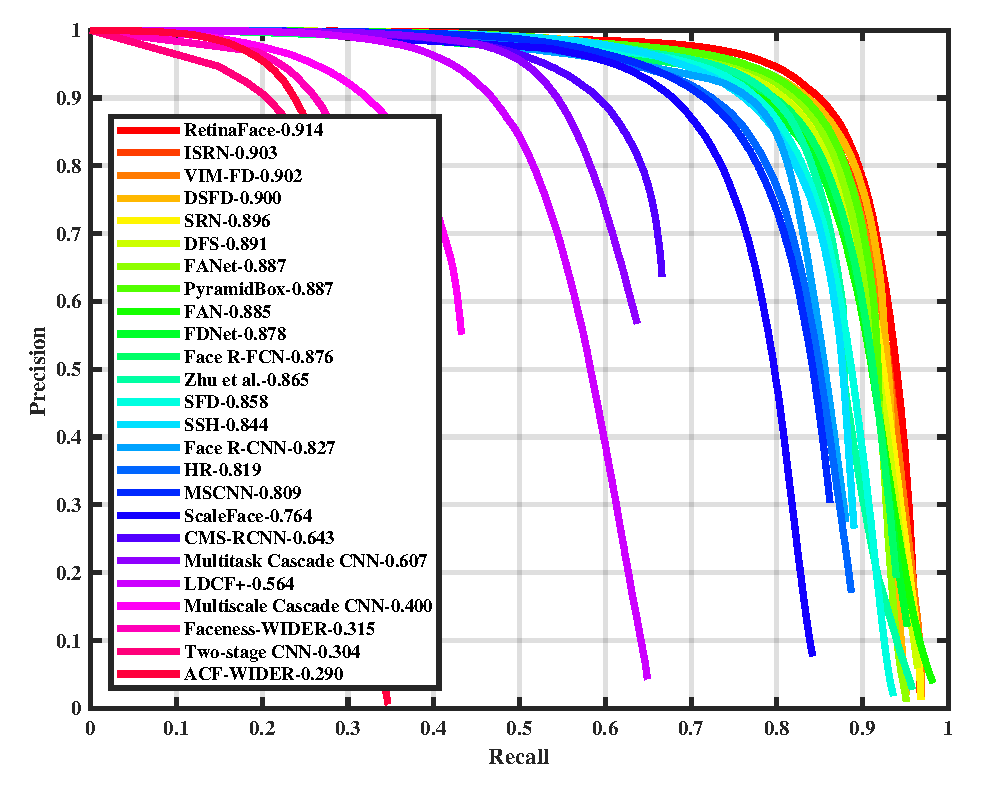
\includegraphics[width=0.32\linewidth]{images/th.pdf}}
        \caption{Đường precision-recall của mô hình RetinaFace trên hai tập dữ liệu val và test của bộ dữ liệu WIDER FACE.}
        \label{fig:wider-face}
    \end{figure*}

    \subsection{Mô hình RetinaFocus}

}

    \facedetectionhighres

    \newpage
    \def\facerecognition{
    \section{Giới thiệu các mô hình giải quyết bài toán Face Recognition}
    \subsection{Giới thiệu các mô hình cổ điển giải quyết bài toán Face Recognition}
    \subsection{Giới thiệu mô hình ArcFace}
}
    \facerecognition

    
    % hello content \cite{test}

    % \newpage


    % \newpage


    % \newpage

    % % KET THUC PHAN NOI DUNG CHINH

    % BAT DAU CAC TRANG CHUC NANG KHAC
    % Xoa header - footer
    \pagestyle{plain}

    \newpage
    \def \tongket{
    \section*{Kết luận và phương hướng phát triển}
    \addcontentsline{toc}{section}{Kết luận và phương hướng phát triển}
    Với sự phát triển của khoa học công nghệ, kích thước của ảnh trong thực tế cuộc sống ngày càng tăng và điều đó đòi hỏi các mô hình học sâu xử lý với độ chính xác cao và tốc độ nhanh.
    Rào cản này đã phần nào đó được vượt qua thông qua các nghiên cứu trong những năm trở lại đây, giúp việc xử lý ảnh chất lượng cao trở nên dễ dàng và chính xác hơn. \\
    Hai đóng góp chính của luận văn bao gồm: \\
    - Mô hình RetinaFocus giúp cải thiện độ chính xác và tốc độ của các mô hình học sâu giải quyết bài toán nhận diện khuôn mặt với trong ảnh chất lượng cao rất nhiều.
    So sánh với mô hình nguyên bản, mô hình RetinaFocus đã tăng tốc ... trong khi duy trì được độ chính xác tương đương trên bộ dữ liệu WIDER FACE. \\
    - Bộ dữ liệu WIDER FACE kích thước lớn đã giúp đánh giá một cách chính xác và khách quan độ chính xác và tốc độ của mô hình RetinaFocus trong việc xử lý ảnh chất lượng cao, so sánh với kết quả của mô hình nguyên bản. \\
    Từ đó, mô hình RetinaFocus sẽ là nền tảng cho các nghiên cứu khác giải quyết bài toán nhận diện khuôn mặt cũng như là nhận diện đối tượng\index{nhận diện đối tượng} trong ảnh chất lượng cao trong tương lai.
}
    \tongket

    \newpage
    \printindex


    % \newpage
    % \def \code{
    % De su dung "pythoncodestyle", ta can `\usepackage{listings}`
    
% De su dung "pythoncodestyle", ta can `\usepackage{listings}`
\def\pythoncodestyle{
    % color and style for code
    \definecolor{codegreen}{rgb}{0,0.6,0}
    \definecolor{codegray}{rgb}{0.5,0.5,0.5}
    \definecolor{codepurple}{rgb}{0.58,0,0.82}
    \definecolor{backcolour}{rgb}{0.95,0.95,0.92}
    \lstdefinestyle{mycodingstyle}{
        backgroundcolor=\color{backcolour},   
        commentstyle=\color{codegreen},
        keywordstyle=\color{magenta},
        numberstyle=\tiny\color{codegray},
        stringstyle=\color{codepurple},
        basicstyle=\ttfamily\footnotesize,
        breakatwhitespace=false,         
        breaklines=true,                 
        captionpos=b,                    
        keepspaces=true,                 
        numbers=left,                    
        numbersep=5pt,                  
        showspaces=false,                
        showstringspaces=false,
        showtabs=false,                  
        tabsize=2
    }
    \lstset{style=mycodingstyle}
}
    \pythoncodestyle

    \section*{Phụ lục}
    \addcontentsline{toc}{section}{Phụ lục}
    \subsection*{Phụ lục 1: Một số đoạn code}
    \subsubsection*{Lập trình Content Encoder}
    \lstinputlisting[language=Python]{codes/content_encoder.py}
    \subsubsection*{Lập trình Style Encoder}
    \lstinputlisting[language=Python]{codes/style_encoder.py}
    \subsubsection*{Lập trình Decoder}
    \lstinputlisting[language=Python]{codes/decoder.py}
    \subsubsection*{Lập trình Generator}
    \lstinputlisting[language=Python]{codes/generator.py}
    \subsubsection*{Lập trình Discriminator}
    \lstinputlisting[language=Python]{codes/discriminator.py}
    \subsubsection*{Lập trình các hàm loss}
    \lstinputlisting[language=Python]{codes/loss.py}
}
    % \code

    \newpage
    \addcontentsline{toc}{section}{Tài liệu tham khảo}
    \renewcommand\refname{Tài liệu tham khảo}
    \bibliography{references.bib}
    \bibliographystyle{unsrt}
    % KET THUC CAC TRANG CHUC NANG KHAC

\end{document}